%\documentclass[a4paper,twoside,12pt]{book}
\documentclass[twoside, openright, 11pt]{report}
\usepackage[spanish]{babel}
\usepackage[utf8]{inputenc}
\usepackage{graphicx} %Para poder insertar las imagenes
\usepackage{float}
\usepackage{listings}
\usepackage{xcolor}
\usepackage[hidelinks]{hyperref}   % optional, nicer for clickable links
\usepackage{geometry} % <-- añadir para ajustar márgenes temporalmente
%\usepackage{url}
%\usepackage{blindtext}

\begin{document}

\begin{titlepage}


\newlength{\centeroffset}
\setlength{\centeroffset}{-0.5\oddsidemargin}
\addtolength{\centeroffset}{0.5\evensidemargin}
\thispagestyle{empty}

\noindent\hspace*{\centeroffset}\begin{minipage}{\textwidth}

\centering

\includegraphics[width=0.9\textwidth]{imagenes/logo_ugr}\\[1.4cm]

\textsc{ \Large TRABAJO FIN DE GRADO\\[0.2cm]}
\textsc{ GRADO DE INGENIERÍA EN INFORMÁTICA}\\[1cm]
% Upper part of the page
%
% Title
{\huge\bfseries NutriPlan\\
}
\noindent\rule[-1ex]{\textwidth}{3pt}\\[3.5ex]
{\large\bfseries Aplicación para la Gestión de Recetas}
\end{minipage}

\vspace{0.5cm}
\noindent\hspace*{\centeroffset}\begin{minipage}{\textwidth}
\centering

\textbf{Autor}\\ {Aissa Rouk El Masoudi}\\[2.5ex]
\textbf{Directores}\\
{CARLOS RODRIGUEZ DOMINGUEZ}\\[2cm]

\includegraphics[width=0.3\textwidth]{imagenes/logo-ceuta.jpg}\\[0.1cm]
\textsc{Facultad de Educación, Tecnología y Economía de Ceuta}\\
\textsc{---}\\
Granada, 15 de Junio de 2025
\end{minipage}
\end{titlepage}
\let\cleardoublepage\clearpage

\chapter*{}
\begin{flushright}
\textit{Dedicado a \\
...}
\end{flushright}
\thispagestyle{empty}

\lstdefinelanguage{TypeScript}{
	keywords={typeof, new, true, false, catch, function, return, null, catch, switch, var, if, in, while, do, else, case, break, export, type, string, number, boolean, interface, extends, implements, import, from, as},
	keywordstyle=\color{blue}\bfseries,
	ndkeywords={class, export, boolean, throw, implements, import, this},
	ndkeywordstyle=\color{teal}\bfseries,
	identifierstyle=\color{black},
	sensitive=true,
	comment=[l]{//},
	morecomment=[s]{/*}{*/},
	commentstyle=\color{gray}\ttfamily,
	stringstyle=\color{green!50!black}\ttfamily,
	morestring=[b]',
	morestring=[b]"
}

\lstset{
	language=TypeScript,
	basicstyle=\ttfamily\small,
	backgroundcolor=\color{gray!10},
	frame=single,
	showstringspaces=false,
	breaklines=true,
	framextopmargin=5pt,
	framexbottommargin=5pt,
	framexrightmargin=5pt,
	columns=fullflexible,
	tabsize=1,
}


\chapter*{Resumen} % si no queremos que añada la palabra "Capitulo"
\addcontentsline{toc}{chapter}{Resumen} % si queremos que aparezca en el índice
\markboth{RESUMEN}{RESUMEN} % encabezado
\thispagestyle{empty}
OMS cita que en 2022 el 43\% de los adultos en el mundo tenía sobrepeso, y el 16\% padecía obesidad, lo que equivale a unos 890 millones de adultos obesos\cite{OMSObesidadySobrepeso}. Desde 1990, el número de personas con obesidad se han más que duplicado entre los adultos y se han cuadruplicado entre los adolescentes\cite{ONUAAComercioAlimentosyObesidad}.
\\Esta situación afecta a personas de todas las edades, regiones y tiene graves consecuencias para la salud, economía y los sistemas sanitarios, hace cada vez más urgente fomentar hábitos alimentarios saludables y estrategias que promuevan una alimentación consciente, eficiente y sostenible.
\\De este contexto surge NutriPlan, una aplicación de Meal Planning y gestión de recetas cuyo objetivo es fomentar un estilo de vida saludable, económico y sostenible, reduciendo el desperdicio de alimentos. 
Esta idea surgió en mi experiencia como estudiante Erasmus, dónde descubrí que al realizar la lista de la compra manualmente y verificar cuáles ingredientes tenía, se ahorraba más dinero en la compra, desperdiciaba menos comida y lo más importante, comía sano.

\chapter*{Abstract} % si no queremos que añada la palabra "Capitulo"
\addcontentsline{toc}{chapter}{Abstract} % si queremos que aparezca en el índice
\markboth{ABSTRACT}{ABSTRACT} % encabezado
\thispagestyle{empty}
This project will proceed with the design and development of a recipe application...

\tableofcontents % indice de contenidos

\cleardoublepage
\addcontentsline{toc}{chapter}{Lista de figuras} % para que aparezca en el indice de contenidos
\listoffigures % indice de figuras

\cleardoublepage
\addcontentsline{toc}{chapter}{Lista de tablas} % para que aparezca en el indice de contenidos
\listoftables % indice de tablas

\chapter{Introducción}\label{cap.introduccion}
  \section{Motivación} 
  Siempre quise crear algo relacionado con mis dos vocaciones, ayudar a las personas y la programación, cada vez que tengo un momento libre intento utilizarlo para pensar cómo hacer el mundo un sitio mejor, qué ideas de aplicaciones podrían aportar algo a las necesidades de la sociedad, esto me llevó a crear varias aplicaciones desde crear una aplicación de escritura reflexiva para mejora personal, hasta la creación de un software administrador de tareas.
  \\
  Esta idea de proyecto surgió cuando estaba en un programa de movilidad estudiantil, después de varios meses realizando la compra e intentando reducir su gasto sin que baje la calidad de mi dieta, noté al principio que cuando realizaba una lista de la compra, gastaba mucho menos de lo que debía, porque no compraba cosas innecesarias o duplicadas. Al cabo de otro tiempo, descubrí que si realizaba mi plan dietético de manera específica antes de realizar la compra semanal, este gasto era mucho menor porque en la lista añadía las cantidades de cada ingrediente que necesitaba, esto no solo redujo mis compras innecesarias, sino que me motivaba a comprar las cantidades exactas necesarias de cada producto o ingrediente, reduciendo el coste de mi compra semanal. 
  \\
  Además de este beneficio económico, percibí que la realización de esta práctica me impulsaba a respetar las cantidades planificadas en mi dieta, haciendo que, esta no solo se volviera más saludable, sino también más variada.
  La Librería Nacional de Medicina Estadounidense realizó un estudio dónde se concluyó que \textit{“la planificación dietética está asociada a una dieta más saludable y una menor prevalencia de obesidad”}\cite{NLMMealPlanningBenefits}, y que \textit{“la práctica de esta podría ser potencialmente relevante para la prevención de la obesidad”}\cite{NLMMealPlanningBenefits}. 
  \\
  Una publicación de la Comisión Europea afirma que los hogares generan más de la mitad del desperdicio alimentario existente y que una de sus causas es la insuficiente planificación de las compras y de las comidas, lo que no solo perjudica la economía familiar, sino que también tiene un impacto ambiental significativo.
  \\
  Todo esto me llevó a crear NutriPlan, una aplicación que satisface todas estas necesidades. Un software que ayuda a los usuarios mediante la creación de una lista de la compra con las recetas ya registradas por el usuario, lleva un seguimiento de su despensa recordando que ingredientes aún tiene disponibles, y calculando cuándo cada ingrediente que se acaba.
  
  \section{Objetivos} 
  El objetivo de este proyecto es la creación de una aplicación móvil que facilite la planificación dietética, haciéndola más sencilla y eficiente promoviendo todos los beneficios discutidos anteriormente en la motivación; lleve un seguimiento de la despensa del usuario y modifique esta cada vez que se realice la compra, planificación de la dieta semanal mediante la adición o eliminación de ingredientes en la despensa.
  \\
  \\
  El resultado será una aplicación con las siguientes funcionalidades:
  
  
  \begin{itemize}
  	\item Gestión de recetas
  	\begin{itemize}
  		\item Adición de una nueva receta mediante la introducción del nombre, enlace, tiempo de preparación y la cantidad de porciones de la receta; la adición de los ingredientes correspondientes a la receta.
  		\item Eliminación o edición de una receta ya existente.
  	\end{itemize}
  	
  	\item Gestión de ingredientes
  	\begin{itemize}
  		\item Adición de nuevos ingredientes a una receta con sus cantidades.
  		\item Posibilidad de buscar (mediante un motor de búsqueda) ingredientes nuevos para añadirlos a una receta que se esté creando.
  	\end{itemize}
  	
  	\item Gestión de dieta semanal
  	\begin{itemize}
  		\item El usuario podrá asignar una o varias recetas para cada comida del día (desayuno, comida, cena), esta asignación es modificable.
  	\end{itemize}
  	
  	\item Gestión de la lista de la compra
  	\begin{itemize}
  		\item El programa será el encargado de la creación de una lista de la compra. Esto se realizará sumando las cantidades de los ingredientes similares de todas las recetas y restando a esta suma las cantidades que haya en la despensa.
  	\end{itemize}
  \end{itemize}
  
  \section{Estructura de la memoria}
  %Explicar de qué va la memoria capítulo por capítulo brevemente
  
  \section{Recursos utilizados}
  
  \section{Planificación temporal}
  

\chapter{Estado del arte}\label{cap.estado del arte}
	\section{Fundamentos}
		\subsection*{La planificación dietética o Meal prepping}
		Hoy en día es difícil tener un estilo de vida saludable dada la falta de tiempo que causan las responsabilidades como el trabajo, familia, sueño, etc; varios datos muestran que los jóvenes consumen mucha menos fruta y verdura de la cantidad recomendada diaria, y que estos consumen mucho más comida basura de la que se recomienda \cite{NLMDifficultyEatingHealthy}.
		\\
		Otro análisis indica que la mayor barrera que impide a las personas de seguir una dieta saludable es la falta de tiempo, el no querer abandonar alimentos favoritos y los elevados precios de las comidas sanas \cite{NLMDifficultyEatingHealthy}. A mucha gente le cuesta mantener ese balance entre trabajar y tener una vida sana y he de ahí donde surge la planificación de dietas o meal planning, una práctica que consiste en planificar las comidas de un periodo futuro determinado (generalmente una semana). La mayor parte de las personas planifican tres comidas por día para los días laborales (de lunes a viernes), pero esta práctica es completamente personalizable.\cite{HowToMealPrep}.
		\\
		\\
		El método de uso de esta práctica puede variar dependiendo de la persona, pero la metodología más común es la siguiente.
		%
		% Pasos para crear una lista de la compra
		%
		\begin{enumerate}
			\item Se elabora una tabla en la que se escriben todos los días de la semana en las columnas y los tipos de comida (desayuno, comida, cena, y en su caso merienda o aperitivo) en las filas  (Figura~\ref{fig:Plantillamealplan}). En cada celda se anotan las recetas o alimentos que se consumirán en el día y la comida correspondiente. A pesar de que este proceso se puede realizar en papel, resulta preferible hacerlo en un ordenador ya que facilita la edición y corrección de posibles errores. La tabla resultante será similar a la de la Figura~\ref{fig:Plantillamealplanrellenada}.
			
			\begin{figure}[H]
				\centering
				\includegraphics[width=1\textwidth]{./imagenes/PlantillaTablamealPlanning.png}
				\caption{Plantilla planificación de comidas}
				\label{fig:Plantillamealplan}
			\end{figure}
			
			\begin{figure}[H]
				\centering
				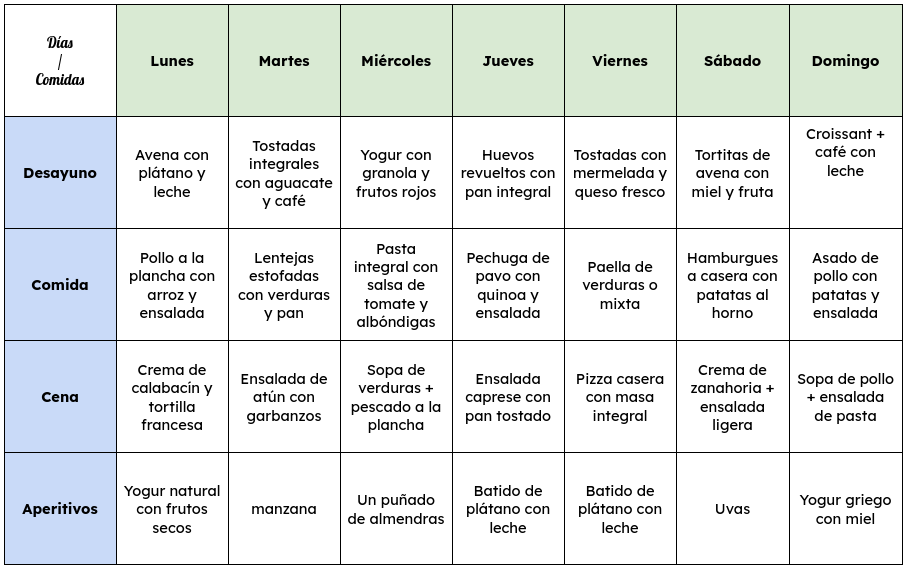
\includegraphics[width=1\textwidth]{./imagenes/PlantillaMealPlanningRellenada.png}
				\caption{Plantilla planificación de comidas}
				\label{fig:Plantillamealplanrellenada}
			\end{figure}
			
			\item Una vez completada la tabla con las recetas de la semana, se procede a listar los ingredientes necesarios para su preparación, incluyendo las cantidades específicas de cada uno (ver Tablas ~\ref{fig:TablaDeIngredientes} y ~\ref{fig:TablaCombinada}).
			
			\begin{table}[H]
				\centering
				\caption{Ejemplo de recetas con ingredientes comunes}
				\begin{tabular}{|p{3.5cm}|p{7cm}|p{3cm}|}
					\hline
					\textbf{Receta} & \textbf{Ingredientes} & \textbf{Cantidad (para 2 personas)} \\ \hline
					Pollo a la plancha con arroz y ensalada &
					Pechugas de pollo, arroz, lechuga, tomate, aceite de oliva, sal, pimienta, limón &
					Pollo 300 g; Arroz 120 g; Lechuga 100 g; Tomate 100 g; Aceite 10 ml \\ \hline
					
					Asado de pollo con patatas y verduras &
					Pollo, patatas, zanahoria, cebolla, aceite de oliva, sal, pimienta &
					Pollo 500 g; Patatas 400 g; Zanahoria 200 g; Cebolla 100 g; Aceite 20 ml \\ \hline
				\end{tabular}
				\label{fig:TablaDeIngredientes}
			\end{table}
			\begin{table}[H]
				\centering
				\caption{Lista de la compra combinada (optimizada)}
				
				\begin{tabular}{|p{5cm}|p{3cm}|}
					\hline
					\textbf{Ingredientes} & \textbf{Cantidad total} \\ \hline
					Pollo & 800 g \\ \hline
					Arroz & 120 g \\ \hline
					Lechuga & 100 g \\ \hline
					Tomate & 100 g \\ \hline
					Patatas & 400 g \\ \hline
					Zanahoria & 200 g \\ \hline
					Cebolla & 100 g \\ \hline
					Aceite de oliva & 30 ml \\ \hline
					Condimentos (sal, pimienta, romero, limón) & Al gusto \\ \hline
				\end{tabular}
			\label{fig:TablaCombinada}
			\end{table}
			
			\item Al obtener la lista de ingredientes necesarios para preparar las recetas planificadas, se revisan los productos disponibles (en el caso de un usuario común, el hogar). Esto permite la identificación de ingredientes que ya se poseen, haciendo que se puedan eliminar de la lista y ajustar la cantidad de los que se tengan parcialmente, evitando compras innecesarias y reduciendo el desperdicio alimentario. En nuestro ejemplo se supondrá que la despensa tiene 500 gramos de pollo y 100 de arroz (Tabla~\ref{fig:TablaCalculoIngr}), dando a la tabla de ingredientes final (Tabla~\ref{fig:TablaIngrFinal}))
			
			% Tabla de ingredientes a comprar y en despensa
			\begin{table}[H]
				\label{fig:TablaCalculoIngr}
				\centering
				\caption{Proceso de cálculo de ingredientes según la despensa}
				\begin{tabular}{|p{3cm}|p{3cm}|p{3cm}|p{3cm}|}
					\hline
					\textbf{Ingredientes} & \textbf{Necesario} & \textbf{En despensa} & \textbf{A comprar} \\ \hline
					Pollo & 800 g & 500 g & 300 g \\ \hline
					Arroz & 120 g & 100 g & 20 g \\ \hline
					Lechuga & 100 g & 0 & 100 g \\ \hline
					Tomate & 100 g & 0 & 100 g \\ \hline
					Patatas & 400 g & 0 & 400 g \\ \hline
					Zanahoria & 200 g & 0 & 200 g \\ \hline
					Cebolla & 100 g & 0 & 100 g \\ \hline
					Aceite de oliva & 30 ml & 0 & 30 ml \\ \hline
					Condimentos & Al gusto & 0 & Al gusto \\ \hline
				\end{tabular}
			\end{table}
		
			% Tabla de ingredientes finales
			\begin{table}[H]
				\centering
				\label{fig:TablaIngrFinal}
				\caption{Lista de la compra final optimizada}
				\begin{tabular}{|p{5cm}|p{3cm}|}
					\hline
					\textbf{Ingredientes} & \textbf{Cantidad a comprar} \\ \hline
					Pollo & 300 g \\ \hline
					Arroz & 20 g \\ \hline
					Lechuga & 100 g \\ \hline
					Tomate & 100 g \\ \hline
					Patatas & 400 g \\ \hline
					Zanahoria & 200 g \\ \hline
					Cebolla & 100 g \\ \hline
					Aceite de oliva & 30 ml \\ \hline
					Condimentos (sal, pimienta, romero, limón) & Al gusto \\ \hline
				\end{tabular}
			\end{table}
		
			
			\item Ahora que se ha obtenido la lista definitiva, es recomendable revisar la lista para ver si falta o se ha duplicado algún ingrediente, este paso no es necesario, pero ayuda a prevenir fallos. Después de esto faltaría solo realizar la compra.
		\end{enumerate}
		%
		%
		En los últimos años la planificación dietética ha ganado popularidad gracias a diversos factores sociales y culturales. De entre ellos destacan el auge de las redes sociales y la creciente influencia del culturismo y el deporte en la vida cotidiana. Plataformas como Instagram, YouTube o TikTok han facilitado el acceso a información sobre estos tópicos, motivando a muchos a estructurar sus dietas de forma más consciente y personalizada. Esta tendencia se observa también en el ámbito deportivo, como por ejemplo en el culturismo, donde el \textit{meal planning} es una práctica habitual y está estrechamente ligada a la preparación física. Varios estudios recientes muestran que los practicantes del culturismo adoptan esta práctica como parte fundamental de su entrenamiento, y que su fuente de información principal son las redes sociales y la comunidad digital \cite{helms2019,masoga2021,benjamins2021}.
		\\
		Este fenómeno no solo se refleja en ámbitos deportivos como el culturismo, sino también en la población general. Una investigación francesa descubrió que el 57,4\% de los habitantes planifican sus comidas al menos de manera ocasional, lo que evidencia un interés extendido en esta práctica como parte de la vida diaria \cite{ducrot2017}. De manera similar, en los Estados Unidos se estima que alrededor del 37\% organizan sus comidas con uno o dos días de antelación, lo que muestra el aumento del uso de la programación de menús fuera del ámbito deportivo \cite{fmi2015}. Esta convergencia entre el impacto social de las plataformas digitales, las prácticas del culturismo y la creciente adopción de \textit{meal planning} en la población aporta una razón y contexto sólidos para el desarrollo de herramientas digitales como \textit{NutriPlan}, cuyo objetivo es facilitar la organización alimentaria de manera sencilla, eficiente y accesible.
		\\\\
		El mercado de aplicaciones de planificación dietética está en constante expansión. Durante 2024 su valor alcanzó los 2,21 millones de dólares y se proyecta que crecerá al valor de 5,53 millones en 2033 \cite{businessresearchinsights2024}. Esta expansión viene impulsada por las nuevas tendencias como la de integración de la inteligencia artificial para la personalización de menús, la incorporación de prácticas sostenibles y la creación de comunidades digitales en torno a la alimentación. Además, la pandemia Covid-19 aceleró esta adopción al fomentar la preparación de comidas en casa y la planificación de las compras. Si se añade a la perspectiva el informe a nivel global de McKinsey, donde se afirma que el 50\% de los consumidores prioriza una alimentación saludable y más del 70\% desea mejorar su dieta, se demuestra un gran interés en este tópico \cite{mckinsey2023}.
		\\\\
		Los beneficios que aporta la planificación dietética son los que generan el interés por este movimiento, caracterizada por la falta de tiempo para funciones básicas como el sueño, la práctica de deporte o la cocina. La organización de comidas no sólo asegura una ingesta calórica y nutricional adecuada, sino que también contribuye en diversos aspectos de la vida diaria.\\
		\textbf{Ahorro de tiempo.} Una de las principales dificultades para mantener hábitos alimenticios saludables es la falta de tiempo. Según análisis hechos por la Biblioteca Nacional de Medicina de EE. UU., esta práctica reduce las compras improvisadas durante la semana y el tiempo empleado en decidir qué cocinar cada día, mejorando la eficiencia y disminuyendo la improvisación.
		\\
		\textbf{Reducción del estrés.} El meal planning ayuda a disminuir la tensión y el estrés derivados de la indecisión diaria sobre qué comer. Muchas personas deciden qué cocinar o comer en momentos de fatiga o poca motivación, lo que les conduce a optar por opciones menos saludables. Disponer de un plan y de los ingredientes necesarios facilita la elección de comidas más equilibradas y reduce la carga mental asociada a esta tarea.
		\\
		\textbf{Mejora de la dieta.} Diversos estudios han demostrado que cocinar en casa con mayor frecuencia se asocia a un consumo menor de carbohidratos, azúcares y grasas \cite{johnshopkins2014}. Además, la planificación dietética incentiva a cumplir objetivos calóricos y nutricionales mediante la compra anticipada de ingredientes. La evidencia científica indica que esta práctica está relacionada con una mejor calidad de dieta y una menor prevalencia de obesidad, lo que la hace potencialmente relevante en estrategias de prevención \cite{ducrot2017}.
		\\
		\textbf{Ahorro económico.} El uso de una lista de la compra estructurada se asocia con una mayor calidad de la dieta y, al mismo tiempo, un gasto más eficiente, ya que evita la adquisición de productos innecesarios \cite{jneb2017}, haciendo que ésta práctica beneficie tanto a la salud como a la economía.
		\\
		\textbf{Reducción del desperdicio alimentario.} Más de 59 millones de toneladas de residuos alimentarios, con un valor estimado en 132 millones; son generados anualmente en la Unión Europea. Una de las principales causas identificadas es la falta de planificación en la compra de alimentos en los hogares \cite{europeancommission2020}. El \textit{meal planning} contribuye en la mitigación de este problema, al fomentar la compra de cantidades ajustadas a las necesidades reales.
	
	
	
	  
	
	\section{Diseño de la interfaz}
		El diseño de la inteefaz de usuario juega un papel muy importante en el uso y la aceptación de la aplicación. De hecho el diseño y usabilidad son requisitos esenciales para el éxito de este tipo de apps \cite{liew2019usability}. Varios estudios señalan que los usuarios tienden a aceptar apps con facilidad de uso, utilidad percibida y calidad de contenido que ofrece la aplicación \cite{Lim2025CuestionarioUsabilidad}. Todo esto demuestra que una interfaz agradable, intuitiva y adaptada a las necesidades del usuario mejora la experiencia de uso de esta y crea un sentimiento positivo hacia la aplicación. Por ello se escogieron varios principios de diseño de interfaz y experiencia de usuario como el diseño minimalista, el uso de colores específicos, etc.
		
		\subsection{Diseño minimalista}
		El disño minimalista es una corriente estética y funcional que se basa en reducir los elementos de una interfaz o producto al mínimo posible sin quitar lo esencial, lo que elimina la información innecesaria y destaca la fundamental. Esta corriente sigue la premisa de "menos es más", frase popular del arquitecto Ludwig Mies van der Rohe, que subraya la importancia de la simplicidad y la funcionalidad en el diseño \cite{wikipediaLessIsMore}. Jakob Nielsen, experti en usabilidad enfatiza que las interfaces deberían evitar la sobrecarga de información, mostrando solo lo esencial \cite{nielsen1994}. Este diseño se basa en los siguientes principios:
		\begin{enumerate}
			\item \textbf{Simplicidad:} mantiene solo los elementos necesarios para comunicar la información.
			\item \textbf{Funcionalidad:} enfatiza que cada componente en el diseño debe tener un propósito claro haciendo que se eliminen elementos decorativos que no aportan ningún propósito claro haciendo que se elmininen elementos decorativos que no aportan ningún valor funcional.
			\item \textbf{Uso de espacio blanco o "negativo":} se usa en la creación de un equilibrio entre los componentes y la redirección de la atención del usuario.
			\item \textbf{Jerarquía visual:} el uso de una jerarquía visual que favorezca y organice la información de manera que los elementos más importantes se destaquen, creando una interfaz navegable y comprensible.
		\end{enumerate}
	\section{Análisis de librerías y frameworks para el frontend y la lógica}
	En este apartado se explican qué son los frameworks y librerías más relevantes utilizados en el proyecto, se presentan las alternativas principales del mercado con sus ventajas e inconvenientes, y se justifica la elección final. Para facilitar la lectura se aborda con detalle React Native y Firebase (pues condicionan arquitectura y despliegue).
	
	\subsection{¿Qué es un framework / librería en este contexto?}
	En el ámbito del desarrollo móvil, un framework es un conjunto estructurado de herramientas, APIs y convenciones que facilita la creación de aplicaciones; una librería es un módulo reutilizable que proporciona funcionalidad concreta (UI, comunicación, almacenamiento, etc.). La elección de framework condiciona la arquitectura, el flujo de trabajo y las opciones de despliegue, mientras que la selección de librerías define aspectos concretos de la experiencia de desarrollo y del producto final.
	
	\subsection{React Native (análisis profundo)}
	React Native es un framework de código abierto propuesto por Meta que permite construir aplicaciones móviles utilizando JavaScript/TypeScript. A diferencia de enfoques híbridos que renderizan UI en un WebView, React Native mapea componentes declarativos a widgets nativos de cada plataforma.
	
	\paragraph{Alternativas principales}
	\begin{itemize}
		\item \textbf{Flutter (Google).} Framework que usa Dart y un motor propio de renderizado; dibuja toda la UI con su propia capa gráfica.
		\item \textbf{Desarrollo nativo (Kotlin/Java para Android, Swift/Objective‑C para iOS).} Máximo control y optimización, código específico por plataforma.
		\item \textbf{Soluciones híbridas (Ionic/Cordova, Capacitor).} Aplicaciones web empaquetadas con acceso a APIs nativas mediante puentes.
	\end{itemize}
	
	\paragraph{Ventajas y desventajas de cada alternativa}
	\begin{itemize}
		\item \textbf{React Native}
		\begin{itemize}
			\item Ventajas: reutilización de código entre plataformas, ecosistema maduro de librerías JS/TS, integración sencilla con módulos nativos, curva de entrada baja para desarrolladores web.
			\item Inconvenientes: en casos de UI muy compleja o rendimiento extremo puede requerir módulos nativos; la coordinación de versiones entre runtime y librerías exige mantenimiento.
		\end{itemize}
		
		\item \textbf{Flutter}
		\begin{itemize}
			\item Ventajas: rendimiento cercano a nativo; control total del rendering; experiencia UI homogénea entre plataformas.
			\item Inconvenientes: requiere aprender Dart y reescribir la UI; menor interoperabilidad directa con bibliotecas JS/TS del ecosistema web existente.
		\end{itemize}
		
		\item \textbf{Desarrollo nativo}
		\begin{itemize}
			\item Ventajas: máximo rendimiento y acceso completo a APIs; ideal para apps con requisitos muy específicos.
			\item Inconvenientes: doble esfuerzo de desarrollo y mantenimiento por plataforma; mayor coste y tiempo.
		\end{itemize}
		
		\item \textbf{Ionic / Cordova / Capacitor}
		\begin{itemize}
			\item Ventajas: desarrollo rápido con tecnologías web; buena opción para apps sencillas.
			\item Inconvenientes: limitaciones de rendimiento y experiencia nativa; comportamiento divergente en gestos y componentes nativos.
		\end{itemize}
	\end{itemize}
	
	\paragraph{Razones para elegir React Native en este proyecto}
	La elección de React Native responde a un equilibrio entre productividad y control técnico: permite desarrollar rápidamente con TypeScript, reutilizar lógica en toda la aplicación y aprovechar un amplio ecosistema (UI kits, navegación, integración con Firebase). Dado el alcance funcional de NutriPlan (formularios, listas, modales, acceso a cámara/galería y persistencia en la nube) React Native ofrece la combinación adecuada de eficiencia de desarrollo y capacidad para escalar con módulos nativos cuando sea necesario.

	\subsection{Otras librerías y componentes}
	
	
	\subsubsection*{Gestión de estado y contexto}
	Dada la complejidad de las aplicaciones y la variedad de componentes es complicado compartir datos entre distintas partes del programa. Un contexto se encarga de pasar información entre diferentes partes y niveles de una aplicación. Existen varias alternativas disponibles para esta función como:
	
	\begin{itemize}
		\item \textbf{React : } módulo de React que permite compartir funciones y estados entre componentes como si fueran variables globales. Es un componente nativo de React y no requiere de dependencias externas, fácil de añadir. Su único inconveniente es que afecta al rendimiento del software si no se planifica bien y no es compatible con estados o efectos complejos.
		\item \textbf{Redux: } librería de código abierto para el manejo de estados en JavaScript que permite mantener un estado globalizado en un componente llamado tienda (\textit{store}) y actualizarlo cuando sea necesario mediante las acciones guardadas en las funciones llamadas \textit{reducers}. Redux permite tener un estado predecible, escalable, fácil de depurar y consistente, pero al mismo tiempo no es un componente nativo de React, es complejo y por ende requiere experiencia y más código de lo usual para configuraciones básicas y excesivo para proyectos pequeños.
		\item \textbf{Zustand: } concepto similar a los anteriores solo que tiene una API muhco más simple que la de redux y un enfoque minimalista. Su simplicidad, flexibilidad, rapidez y no necesidad de \textit{wrappers} como \texttt{React Context} le hacen eficiente y fácil de utilizar.
	\end{itemize}

	Se ha usado \texttt{React Context} para el uso del contexto gracias a su facilidad de instalación, que se realiza en un sólo comando; su simplicidad y al tener una aplicación no tan compleja, esta librería no afectaría en el rendimiento.
	
	\subsubsection*{Navegación}
	La navegación en este caso es necesitada para la conexión entre pantallas permitiendo al usuario acceder a todo el contenido de la aplicación en un orden específico.  Existen varias alternativas como:
	
	\begin{itemize}
		\item \label{ReactNativeNavigation}
		\textbf{React Native Navigation}: librería creada por \textit{React Native} que permite la navegación e implementación de pilas (\textit{stack}), pestañas y bandejas de navegación, se integra con gestos y la navegación nativa de React Native, es fácil de utilizar, pero menos eficiente en grandes proyectos.
		\item \textbf{React Native Navigation(Wix)}: a diferencia de \textit{React Native Navigation} que usa JavaScript, esta usa las API nativas de navegación de iOS y Android, es más eficiente en grandes proyectos pero difícil de configurar.
	\end{itemize}
	
	Al estar trabajando en un proyecto simple que no requiere de muchas páginas ni tampoco utiliza pestañas o bandejas de navegación se ha utilizado \textit{React Native Navigation} para controlar las pantallas y su acceso dada su simplicidad de uso, fama y eficiencia en programas pequeños.
	
	\subsubsection*{\texttt{@rneui/themed} (React Native Elements) y UI kits}
	Conjunto de componentes de interfaz listos para usar (botones, inputs, cards, etc.).  
	Alternativas: React Native Paper, NativeBase, UI Kitten.  
	Ventajas: aceleración en la construcción de pantallas, tematización central, componentes coherentes. Inconvenientes: peso adicional en la app y limitaciones si se requiere personalización extrema.  
	Razón de elección: \texttt{@rneui/themed} proporciona los componentes que mejor encajan con el estilo requerido y permite personalizaciones sencillas sin reescribir elementos base; se usa en varios componentes del proyecto.
	
	\subsubsection*{Búsqueda local: \texttt{react-minisearch} (MiniSearch)}
	Motor de búsqueda en memoria ligero para texto indexa documentos y permite búsquedas por prefijo y ranking.  
	Alternativas: Fuse.js (búsqueda difusa), Lunr.js (índice invertido similar a motores más grandes).  
	Ventajas: MiniSearch es muy ligero, simple de integrar y suficiente para listas pequeñas/medianas como el catálogo de ingredientes. Inconvenientes: no diseñado para grandes volúmenes o búsqueda distribuida.  
	Por qué se escogió: en \texttt{IngredientSearchSelectorComponent} en la app se requiere latencia mínima y funcionamiento offline; MiniSearch satisface estos requisitos con bajo coste.
	
	\subsubsection*{Iconos: \texttt{react-native-vector-icons} (Ionicons)}
	Colección de iconos vectoriales para React Native con adaptadores para múltiples familias (Ionicons, Material, etc.).  
	Alternativas: usar SVGs con \texttt{react-native-svg}, o iconos del sistema.  
	Ventajas: fácil uso, consistencia visual y escalabilidad; amplia disponibilidad de glyphs. Inconvenientes: usado en cabeceras y botones.
	
	\subsubsection*{Pickers y selectores: \texttt{CustomPicker} y bibliotecas}
	Es un componente local \texttt{\hyperref[CustomPicker]{CustomPicker}} que abre un \texttt{Modal} con opciones para seleccionar el \texttt{quantityType}(unidad de métrica del ingrediente).
	Alternativas: \texttt{@react-native-picker/picker} (nativo) o \texttt{react-native-dropdown-picker} (más características).  
	Ventajas del enfoque actual: control total sobre la apariencia del modal y la interacción; comportamiento consistente en iOS/Android. Inconvenientes: requiere implementar accesibilidad y animaciones manualmente.  
	Razón de elección: necesidad de un comportamiento visual concreto integrado en \texttt{IngredientComponent} y de un control simple sobre apertura/cierre mediante las props \texttt{isPickerOpen} / \texttt{setIsPickerOpen}.
	
	
	
	\subsubsection*{Imágenes y selección de medios}
	Librería de gestión de imágenes mediante bibliotecas nativas (por ejemplo \texttt{react-native-image-picker}).  
	Alternativas: Expo Image Picker, soluciones servidoras.  
	Ventajas: acceso nativo a cámara/galería y control de permisos. Inconvenientes: configuración nativa inicial.  
	Razón: se eligió la solución que ofrece más control sobre permisos y procesado de imágenes en la ejecución nativa, no se puede utilizar la opción de \textit{Expo} ya que le proyecto no fué programado de manera nativa.
  
  
	\section{Análisis de librerías y frameworks para back-end}
		
		\subsection{Base de datos}
		Es el software encargado de guardar todos los datos necesarios del usuario y tenerlos al alcance en cualquier momento. Existen varias opciones que cubren nuestras necesidades, desde bases de datos locales hasta en la nube.
		\begin{itemize}
			\item \textbf{SQLite.} Es una base de datos relacional autónoma y ligera que es usada en proyectos locales y en línea; utiliza SQL como su lenguaje de programación, su instalación en \textit{React Native} es fácil e intuitiva. A pesar de que SQLite tiene esos beneficios, su integración en aplicaciones que necesitan bases de datos en la nube resulta complicado y costoso dado que SQLite no incorpora de forma nativa la sincronización de datos online.
			%
			\item \textbf{Firebase.} Plataforma creada por Google que integra servicios de autenticación, bases de datos en tiempo real, almacenamiento de ficheros, y herramientas auxiliares para análisis y despliegue. La mayor parte de sus servicios son gratuitos(hasta superar un límite establecido), a pesar de que su base de datos no sea relacional, no resulta difícil usarla como tal; su integración con \textit{React Native} se realiza en varios pasos y es muy simple; y por último tiene una comunidad muy grande que aporta documentación y \textit{feedback} extenso. En cuento a sus desventajas, estas son el no ser óptimo en relaciones o búsquedas complejas y su pago.
			%
			\item \textbf{SupaBase. } Base de datos de código abierto que utiliza 
			\textit{PostgreSQL} haciéndola muy robusta y potente, tiene atuenticación almacenamiento y funciones serverless(no requieren de servidor) y es gratuito gracias a su filosofía de código abierto. En cambio, no es tan maduro ni ampliamente probado en aplicaciones móviles (no tanto como Firebase), tiene una configuración e uso complejo y técnico y su documentación no es tan extensa.
			\item \textbf{MongoDb. } Base de datos local que contiene sincronización nativa con la nube, resulta óptima para aplicaciones que requieren de almacenamiento en y sin línea (online y offline) y el tipo de base de datos es similar al de \textit{Firebase}(no relacional). Sin embargo, su uso resulta complejo al añadir lógica personalizada al backend, no tiene una comunidad tan madura con React Native.
		\end{itemize}
	
		Para el backend se necesita una base de datos para una aplicación que no consume, no contiene muchos datos; que la base de datos sea minimalista en el aspecto del uso e instalación, pensada para app móviles y no tenga ningún coste económico. Firebase cumple con todas estas condiciones y además contiene servicios de autenticación y reglas de seguridad, por ello se escogió este como software de almacenamiento.
		
		
  	
	\section{Proyectos actuales}
	%Nombrar aplicaciones que hayan resultado de inspiración para el proyecto y explicar un poco de qué van esas aplicaciones
	  % ...existing code...
		\subsection*{Aplicaciones móviles existentes de meal planning}
		El interés creciente por planificar la alimentación doméstica ha dado lugar a aplicaciones con enfoques bien diferenciados: desde soluciones orientadas a la rapidez y conveniencia hasta plataformas centradas en el control nutricional o en la compra integrada. A continuación se exponen las diferencias esenciales entre las propuestas comerciales más conocidas y NutriPlan.
		
		\begin{itemize}
			\item \textit{\textbf{Mealime}} apuesta por la simplicidad y la velocidad: menús semanales preconfigurados y listas de compra automáticas reducen la fricción para el usuario que busca solucionar comidas sin preocuparse por detalles. Esa filosofía simplifica la adopción inicial pero sacrifica flexibilidad; las recetas y porciones estandarizadas limitan la capacidad de ajustar ingredientes, sustituir productos o conciliar con el inventario real del hogar. Para una herramienta cuyo valor diferencial es precisamente optimizar la lista de la compra en función de la despensa, esa pérdida de precisión es significativa.
			
			\item \textit{\textbf{Yazio}} sitúa el foco en el seguimiento nutricional: ofrecer conteo calórico y trazabilidad de macronutrientes requiere una base de datos nutricional rica y una interfaz que guíe al usuario en la introducción y el ajuste de datos. Es una excelente opción para objetivos de salud, pero su complejidad y el uso extendido de funciones premium añaden barreras de entrada. En el contexto de este proyecto, donde la prioridad es validar un flujo práctico (receta → planificación → despensa → lista) la profundidad nutricional extrema no aporta tanto valor inmediato como la fiabilidad en el cálculo de la compra y la experiencia off‑line.
			\item \textit{\textbf{Instacart}} se orienta hacia la transacción: conecta recetas y menús con la compra directa en supermercados asociados. Su fortaleza es la integración comercial y la comodidad para comprar en pocos pasos; su limitación es la dependencia de cobertura regional y acuerdos con comercios, además de que el objetivo principal es la venta más que la personalización dietética o la reducción del desperdicio.
		\end{itemize}
		  
		Frente a estos enfoques, NutriPlan se diseñó con prioridades claras y deliberadas: ofrecer control granular sobre las recetas, garantizar la conciliación precisa con la despensa del usuario, funcionar con baja latencia (incluso sin conexión) y mantener la propiedad y privacidad de los datos. Estas prioridades se tradujeron en decisiones técnicas y de producto concretas:
		
		\begin{itemize}
			\item \underline{Precisión y granularidad:} cada receta modela ingredientes con cantidad y unidad (\texttt{RecipeIngredient} en \texttt{src/Types/Types.tsx}), lo que permite cálculos exactos para la lista de la compra. Aunque exige mayor entrada de datos por parte del usuario, reduce el desperdicio y mejora la utilidad práctica del sistema.
			
			\item \underline{Disponibilidad y rendimiento:} la indexación local (MiniSearch) y la persistencia de Firestore proporcionan búsquedas instantáneas y operación offline para tareas frecuentes, mejorando la experiencia en contextos reales como tiendas con cobertura limitada.
			
			\item \underline{Privacidad y propiedad de datos:} los datos se aíslan por usuario (\texttt{uid}) y las reglas de seguridad de Firestore protegen la información personal; esta opción refuerza la confianza del usuario y facilita la portabilidad de los datos.
			
			\item \underline{Modelado equilibrado para BaaS:} el diseño de datos combina referencias y elementos embebidos para minimizar lecturas innecesarias en Firestore y mantener pantallas reactivas (p. ej. \texttt{MainScreen}, \texttt{GroceryListScreen}), reduciendo costes operativos y latencia.
			
			\item \underline{Onboarding progresivo y usabilidad:} la experiencia se organiza para que el usuario comience con tareas esenciales (añadir recetas, planificar, generar lista) y pueda acceder a funcionalidades más complejas solo si lo desea; la interfaz usa modales y componentes reutilizables (\texttt{src/Components/}) para minimizar el esfuerzo cognitivo.
			
			\item \underline{Modularidad y evolución:} la separación en capas (Components, Screens, Services, Context, Types) permite validar la idea con rapidez y mantener la puerta abierta a integraciones futuras (APIs de supermercados, motores de recomendación, o servicios avanzados de nutrición) sin reescribir la interfaz.
		\end{itemize}
		
			
			En conjunto, NutriPlan se sitúa entre las aplicaciones sencillas orientadas a la conveniencia y las plataformas complejas centradas en la nutrición o en el comercio electrónico. La elección de priorizar precisión en las recetas, conciliación con la despensa y operación offline responde a un objetivo práctico: reducir desperdicio y ofrecer una herramienta útil en el día a día del usuario. Estas decisiones, aunque aumentan la complejidad técnica inicial, maximizan el valor real entregado y facilitan evolucionar la aplicación hacia funcionalidades adicionales cuando la validación con usuarios lo aconseje.

	\section{Conclusiones}
	%Análisis propio (sin referencias bibliográficas) de lo que el autor considera sobre todo lo que ha explicado en el apartado de "Estado del arte". En nuestro caso, considerar qué librería es mejor que otra y en qué aspectos
	Tras analizar las distintas tecnologías y herramientas disponibles para el desarrollo de aplicaciones móviles, especialmente en el contexto de la planificación de comidas, podemos extraer conclusiones relevantes sobre las decisiones tomadas en este proyecto:
	
	\subsection*{Frameworks de desarrollo móvil}
	React Native ha demostrado ser la elección más adecuada frente a alternativas como Flutter o desarrollo nativo puro. Sus principales ventajas radican en:
	\begin{itemize}
		\item La capacidad de mantener una única base de código para iOS y Android, reduciendo significativamente el tiempo de desarrollo.
		\item Un ecosistema maduro de librerías que facilita la implementación de funcionalidades comunes.
		\item La posibilidad de aprovechar el conocimiento previo de JavaScript/TypeScript y React.
	\end{itemize}
	
	Sin embargo, es importante reconocer que Flutter podría ofrecer mejor rendimiento en aplicaciones con interfaces muy complejas o animaciones elaboradas. No obstante, para las necesidades de NutriPlan, donde prima la funcionalidad práctica sobre efectos visuales complejos, React Native proporciona el balance óptimo entre velocidad de desarrollo y rendimiento.
	
	\subsection*{Backend as a Service (BaaS)}
	Firebase ha resultado ser superior a alternativas como Supabase o un backend personalizado para este proyecto específico por:
	\begin{itemize}
		\item Facilidad de integración con React Native mediante SDKs oficiales.
		\item Capacidades de sincronización offline que mejoran la experiencia del usuario.
		\item Reducción significativa en tiempo de desarrollo al no requerir infraestructura propia.
	\end{itemize}
	
	Aunque las demás opciones ofrecen ventajas en términos de código abierto y control sobre los datos, Firebase proporciona una solución más madura y probada para las necesidades actuales de la aplicación. La decisión de usar Firestore sobre Realtime Database se justifica por su modelo de datos más flexible y mejor soporte para consultas complejas.
	
	\subsection*{Gestión de estado}
	La elección de React Context sobre alternativas como Redux o MobX se fundamenta en:
	\begin{itemize}
		\item Simplicidad en la implementación y menor curva de aprendizaje.
		\item Suficiente para la escala actual de la aplicación.
		\item Integración nativa con React sin dependencias adicionales.
	\end{itemize}
	
	Si bien Redux ofrece ventajas en aplicaciones más grandes, especialmente en términos de depuración y manejo de estados complejos, la sobrecarga que introduce no se justifica para el alcance actual de NutriPlan.
	
	\subsection*{Navegación y ruteo}
	React Navigation ha demostrado ser superior a alternativas como React Native Navigation (Wix) en nuestro caso por:
	\begin{itemize}
		\item API más intuitiva y documentación más completa.
		\item Mejor integración con el ecosistema React Native.
		\item Soporte nativo para gestos y animaciones en iOS y Android.
	\end{itemize}
	
	\subsection*{UI Components}
	La combinación de React Native Elements (@rneui/themed) con componentes personalizados ha resultado más efectiva que usar soluciones completas como Native Base o UI Kitten porque:
	\begin{itemize}
		\item Permite mayor flexibilidad en el diseño de la interfaz.
		\item Reduce el tamaño final de la aplicación al incluir solo los componentes necesarios.
		\item Facilita la personalización y consistencia visual.
	\end{itemize}
	
	\subsection*{Búsqueda y rendimiento}
	La implementación de búsqueda local con MiniSearch ha demostrado ser más eficiente que alternativas como Fuse.js o búsquedas en servidor por:
	\begin{itemize}
		\item Mejor rendimiento en búsquedas sobre conjuntos de datos medianos.
		\item Funcionamiento offline sin depender de la red.
		\item Menor consumo de recursos del dispositivo.
	\end{itemize}
	
	\subsection*{Conclusión general}
	Las decisiones tecnológicas tomadas priorizan tres aspectos fundamentales:
	\begin{enumerate}
		\item Velocidad de desarrollo y prototipado rápido.
		\item Experiencia de usuario fluida con buen rendimiento offline.
		\item Mantenibilidad y escalabilidad del código.
	\end{enumerate}
	
	Aunque existen alternativas que podrían ofrecer ventajas en aspectos específicos (rendimiento puro, control total sobre el backend, capacidades avanzadas de estado), las elecciones realizadas proporcionan el mejor compromiso para los objetivos del proyecto: crear una aplicación funcional, mantenible y con buena experiencia de usuario, permitiendo iteraciones rápidas y validación de funcionalidades con usuarios reales.

\chapter{Diseño y descripción del sistema}\label{cap.diseno y descripcion del sistema} %En este apartado se detallarían decisiones de diseño e implementación, como la decisión de utilizar React-Native y explicar por qué se ha elegido ese motor sobre otros
	\section{Lógica de la aplicación}
		\subsection{Decisiones de diseño: estructura, clases y casos de uso}
			En esta sección se explica de forma explícita y concisa qué decisiones de diseño se adoptaron en la aplicación y por qué se tomó cada una de ellas.
		
		
		\subsection{Casos de uso}
			\label{sec:casos_de_uso}
			
			En esta sección se enumeran y justifican los casos de uso principales de la aplicación \textit{NutriPlan}. Cada caso de uso incluye la motivación para su inclusión en el sistema, la forma en que se materializó en la implementación (referencias a módulos y ficheros relevantes) y una discusión sobre alternativas de diseño que se valoraron durante el desarrollo, explicando por qué la solución adoptada resultó la más adecuada para los objetivos del proyecto.
		
		\subsubsection*{Criterio de selección de los casos de uso}
			Los casos de uso se seleccionaron atendiendo a los requisitos funcionales básicos y a las prioridades del proyecto: permitir al usuario planificar sus comidas semanalmente, gestionar recetas e ingredientes, mantener un inventario de despensa y obtener una lista de la compra optimizada. Se dio preferencia a casos que maximizaran el beneficio al usuario final y que fueran implementables con un coste razonable de desarrollo.
		
		\subsubsection{1. Registro e inicio de sesión}
			La mayoría de aplicaciones permiten al usuario a crear una cuenta, iniciar sesión y mantener esta activa en el dispositivo. Esto es esencial para la separación de datos entre diferentes cuentas desde recetas privadas, despensas e planificaciones.\\
			Para ello la manera más sencilla y eficiente de implementar este caso de uso es mediante la creación de las pantallas de inicio y registro de sesión (\textit{LoginScreen} e \textit{RegisterScreen}) que permitan al usuario registrarse e iniciar sesión y mantener la cuenta activa en su dispositivo.\\
			Su implementación es con Firebase que proporciona \textit{Firebase Auth} que permite controlar el inicio de sesión y la autenticación.\\
			Existen varias alternativas que satisfacerían estos casos de us como la autenticación mediante un backend propio (REST/API) o servicios como Auth0. Estos se descartaron por la sobrecarga operativa y de configuración; Firebase ofrece integración directa con React Native, SDKs maduros y un tiempo de puesta en marcha muy inferior, adecuado para un TFG cuyo objetivo es priorizar la funcionalidad de cara al usuario.
		
		\subsubsection{2. Gestión de recetas (CRUD)}
			El componente más importante de nuestra aplicación es la receta y como en cada lista, el usuario tiene el derecho de crear, editar, eliminar, programar y listar las recetas con sus ingredientes y metadatos.\\
			Para ello se ha creado una arquitectura en la base de datos que separa entidades, funciones CRUD que comunican con la base de datos; pantallas y modales que muestran y permiten la edición de estos
		
		\subsubsection{3. Búsqueda de ingredientes y selección rápida}
			Ofrecer una búsqueda rápida de ingredientes para añadir a recetas o planificaciones. Para ello se creó una barra de búsqueda y se usó \textit{mini-search} como motor de búsqueda. Una búsqueda rápida y disponible offline mejora notablemente la experiencia de creación de recetas. Indexar en cliente reduce latencia y dependencia de la red en tareas frecuentes.\\
			Hay alternativas como búsquedas remotas (consultas a Firestore, o un servicio externo) o usar Fuse.js. Se prefirió MiniSearch por su rendimiento y simplicidad cuando los volúmenes de datos son pequeños/medios; la búsqueda remota hubiera incrementado latencias y coste de lecturas.
		
		\subsubsection{4. Planificación semanal de comidas}
			Como lo usual en cada planificación de menús, se tiene que poder asignar recetas o ingredientes a días y comidas (desayuno/comida/cena) y visualizar la semana con las asignaciones.  
			Para la Implementación de este caso se usan vistas (\textit{View}) en \texttt{MainScreen} como orquestador, \texttt{HeaderComponent} para selección del día y servicios \texttt{weeklyMeals-db-services.ts} para conectar con Firebase.\\
			Centralizar la planificación en \texttt{MainScreen} permite ofrecer una vista de contexto (lista de recetas previstas, botones de acción) y mantener la interacción rápida mediante modales para planificar. Se diseñó la entidad \texttt{WeeklyMeal} con campos mínimos que permiten tanto enlazar a una receta como a un ingrediente suelto.  
			Alternativas: sistema de planificación basado en reglas (p. ej. sugerencias automáticas por variedad nutricional) o planificación mediante calendarios externos. Estas ideas quedaron fuera del alcance inicial por aumentar la complejidad; se mantienen como mejoras futuras.
		
		\subsubsection{5. Gestión de despensa (inventario)}
			Uno de los beneficios de esta aplicación es la característica de mantener un inventario local con los ingredientes disponibles, actualizarlos en cualquier momento y hacer el cálculo automático de los ingredientes necesarios después de restar los presentes.
			Para ello, la implementación de \texttt{PantryScreen}, \texttt{ingredientPantry-db-services.ts} y componentes de tarjeta (\texttt{PlannedIngredientCard}, \texttt{IngredientCard}) para la visualización y el cálculo de los ingredientes planificados.  
			La despensa es clave para calcular la lista de la compra optimizada; por ello se optó por un modelo sencillo (\texttt{PantryItem}) que almacena cantidad y unidad por usuario. Las operaciones de suma/resta se realizan en servicios para mantener lógica centralizada, otras alternativas serían la sincronización exclusiva con supermercado (APIs externas) o almacenamiento solo en servidor. Se optó por persistencia con Firestore y caching local para permitir uso offline y reducir latencias.
		
		\subsubsection{6. Generación y gestión de la lista de la compra}
			Calcular la cantidad a comprar sumando ingredientes planificados y restando existencias en la despensa; marcar artículos como comprados.\\
			Implementación mediante la creación de \texttt{GroceryListScreen} para la muestra de los ingredientes a comprar, \texttt{groceryBought-db-services.ts} para la conexión con Firebase y \texttt{GroceryItem} que determina la estructura de los datos.
			Automatizar el cálculo de la lista de la compra es el valor diferencial central del producto. Al implementar este cálculo en la capa de servicios se asegura consistencia y evita duplicación de lógica en la UI. Marcar como comprado actualiza la despensa mediante operaciones atómicas o lotes para evitar desajustes.  
			Se podía haber delegado el cálculo en un backend propio o en funciones serverless para mayor control. Se valoró, pero se priorizó la simplicidad operativa aprovechando Firestore y la capacidad de operaciones por lotes en clientes.
		
		\subsubsection{7. Gestión de imágenes y multimedia}
			Descripción: permitir asociar imágenes a recetas y gestionar permisos de cámara/galería.  
			Implementación: subida a Firebase Storage y almacenamiento de \texttt{imageUrl} en documentos de receta; componentes que usan \texttt{react-native-image-picker}.  
			Justificación: imágenes mejoran la usabilidad y ayudan al reconocimiento visual de recetas; Firebase Storage facilita el almacenamiento y entrega CDN‑like.  
			Alternativas: almacenar imágenes como base64 en documentos o usar servicios externos de CDN; se descartaron por coste y complejidad de integración.
		
		\subsubsection*{Resumen y coherencia de los casos de uso}
			Los casos de uso seleccionados cubren el flujo completo esperado por el usuario: registrar y acceder a su cuenta, crear y organizar recetas, planificar menús, verificar la despensa y generar la lista de la compra. Cada caso se implementó priorizando latencia baja, disponibilidad offline y simplicidad de mantenimiento: decisiones que se reflejan en la estructura de ficheros (\texttt{src/Services/}, \texttt{src/Screens/}, \texttt{src/Components/}) y en el modelado de datos (\texttt{src/Types/Types.tsx}). Las alternativas más complejas (backend propio, normalización extrema, trazabilidad con Redux) se consideraron pero se descartaron por coste de desarrollo o por no aportar suficiente ventaja en la fase inicial del proyecto. Estas decisiones dejan, no obstante, margen para futuras migraciones y escalado cuando los requisitos lo exijan.
		
		
			\clearpage
			\newgeometry{left=0cm,right=0cm,top=5cm,bottom=0cm} 
			\thispagestyle{empty}
			\noindent
			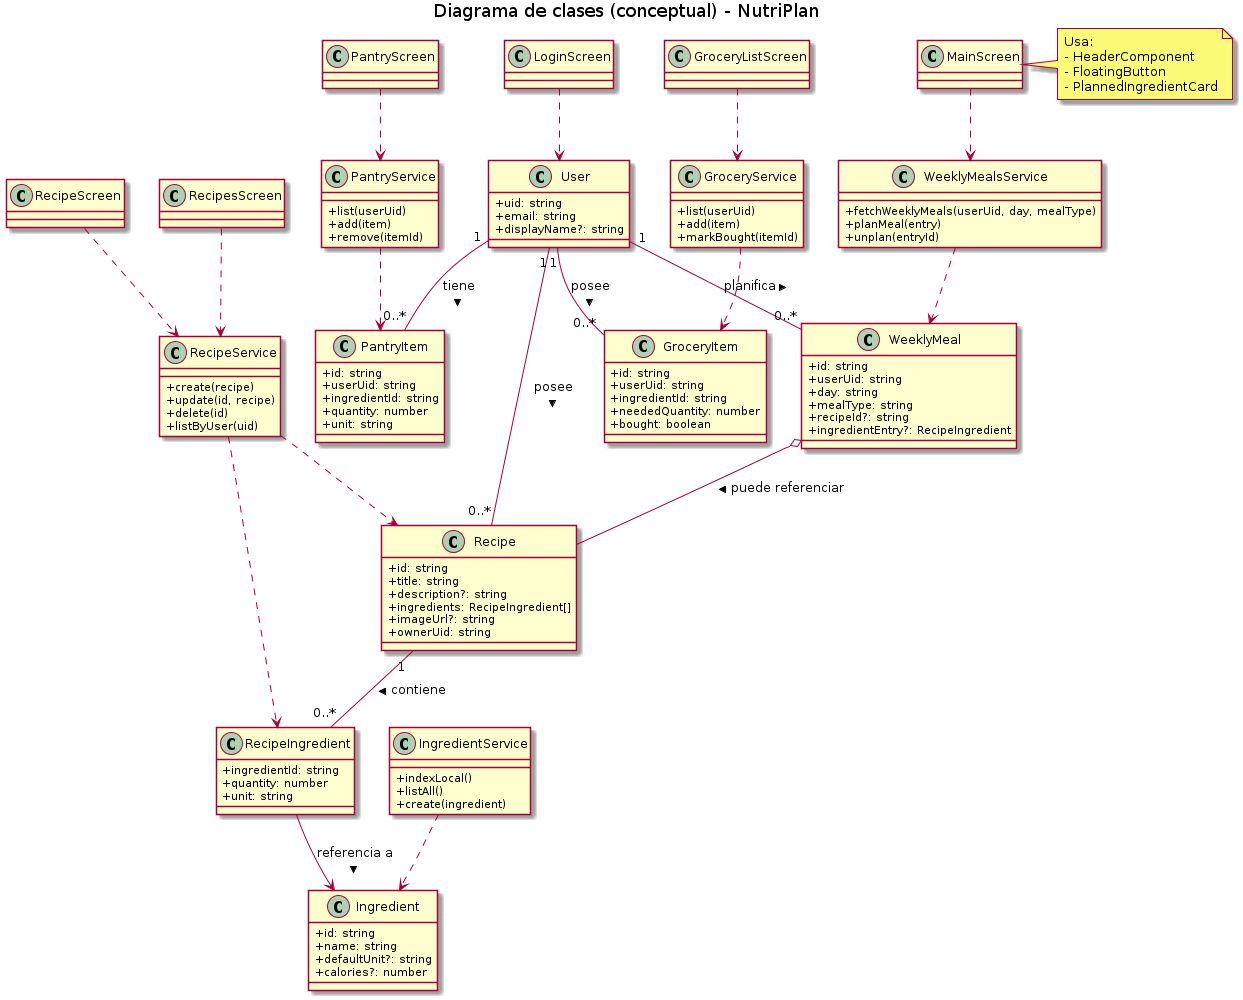
\includegraphics[width=\paperwidth,height=\paperheight,keepaspectratio]{imagenes/class_diagram}
			\clearpage
			\restoregeometry
		
		\subsection{Justificación del diagrama de clases y decisiones de diseño}
		\label{sec:justificacion_diagrama}
		
			En este apartado se justifican las decisiones que motivaron la separación representada en el diagrama de clases conceptual y se explica por qué cada componente, clase y relación fue diseñada de la manera mostrada.
			
			\subsubsection{Criterio general de separación}
				La arquitectura sigue un principio de separación por responsabilidades (single responsibility, bajo acoplamiento y alta cohesión). Se decidió distinguir claramente entre:
				\begin{itemize}
					\item Entidades del dominio llamadas tipos en \textit{TypeScript} que son similares a las clases (tipos que modelan los datos): representan la forma y semántica de los objetos (User, Recipe, Ingredient, RecipeIngredient, WeeklyMeal, PantryItem, GroceryItem).
					\item Servicios por dominio (capa Services): encapsulan la lógica de persistencia y las operaciones con la base de datos de Firebase.
					\item Vistas/controladores (Pantallas y Componentes): orquestan flujos de interacción y presentan datos al usuario.
					\item Contexto y tipado (Context / Types): comparten estado global y contratos tipados entre capas.
				\end{itemize}
				Esta separación permite modificar la fuente de datos (por ejemplo migrar Firebase por otro BaaS) sin cambiar la UI, facilita la escritura de pruebas unitarias y simplifica la localización de la lógica de negocio.
			
			\subsubsection{Entidades del dominio: elección de atributos}
				Las entidades modeladas en \texttt{Types.tsx} recogen únicamente los atributos necesarios para las operaciones de la aplicación, siguiendo criterios de minimalismo y practicidad.
			
				\begin{itemize}
					\item \textit{\underline{User}} (usuario): uid, email, displayName.  
					Razonamiento: el identificador único (uid) es la clave primaria en Firebase y es suficiente para asociar propiedad y seguridad. Los metadatos se reducen al mínimo imprescindible (email y nombre para mostrar).
					Otras opciones consideradas: añadir perfil extenso (roles, preferencias nutricionales). Se descartó por simplicidad y porque esas extensiones sólo se exigirán si el caso de uso lo demanda.
					
					\item \label{Recipe}
					\textit{\underline{Recipe}} (Receta): id, title, description, ingredients[], imageUrl, ownerUid.  
					Razonamiento: una receta requiere un identificador, metadatos visibles (título, descripción), referencia al propietario para control de acceso y lista de ingredientes embebidos (RecipeIngredient) para renderizado rápido. ImageUrl se almacena como referencia a Firebase Storage.
					Alternativas: normalizar completamente los ingredientes (referencias sólo a ids) para evitar duplicación. Se escogió un balance: almacenar RecipeIngredient con referencia al ingredientId y cantidades, lo que permite reconstruir la receta sin múltiples consultas complejas y mantiene integridad semántica.
					
					\item \label{Ingredient}
					\textit{\underline{Ingredient}} (Ingrediente): id, name, defaultUnit, calories.  
					Razonamiento: ingredientes tienen nombre y unidad por defecto; valores nutricionales se guardan opcionalmente. Mantener metadata ligera facilita indexación local (MiniSearch).
					Alternativas: modelo extensible con tablas de nutrición completas. Se reservó para iteraciones futuras.
					
					\item \textit{\underline{RecipeIngredient}} (Ingrediente de receta): ingredientId, quantity, unit.  
					Razonamiento: estructura que refleja la relación entre receta e ingrediente con cantidad y unidad. Este tipo evita ambigüedades y permite operaciones aritméticas (sumas para la lista de la compra).
					Alternativas: modelo por ítem sin referencia (texto libre). Se desechó por perder control en cálculos y agregaciones.
					
					\item \textit{\underline{WeeklyMeal / PantryItem / GroceryItem}}: campos mínimos para identificar usuario, entidad referenciada, cantidad, unidad y estado.  
					Razonamiento: el foco es soportar planificación, inventario y compras; por ello se incluyeron únicamente atributos necesarios para esas operaciones.
				\end{itemize}
			
			
				En todos los casos se priorizó la claridad semántica y la operatividad (facilidad de cálculo de listas de compra, conciliación con la despensa y sincronización con Firebase).
			
			\subsubsection{Relaciones entre entidades: multiplicidad y tipo}
				Las decisiones sobre multiplicidad (p. ej. User 1 -- 0..* Recipe) reflejan la realidad del dominio:
				\begin{itemize}
					\item Un usuario puede poseer muchas recetas; una receta pertenece a un único propietario (ownerUid).
					\item Una receta contiene múltiples RecipeIngredient; cada RecipeIngredient referencia un Ingredient.
					\item WeeklyMeal puede referenciar una Recipe o un RecipeIngredient (soporte tanto para planificar por receta como para planificar por ingrediente suelto).
				\end{itemize}
				Se eligieron relaciones que favorecen consultas eficientes en Firestore (documentos con colecciones anidadas o referencias) y disminuyen la necesidad de joins costosos en el cliente.
			
				Alternativas de modelado consideradas:
				\begin{itemize}
					\item Modelado completamente normalizado (separar por completo recetas/ingredientes y usar solo referencias). Pro: evita duplicación; Contra: aumenta número de lecturas y complejidad en tiempo de ejecución en un BaaS tipo Firestore.
					\item Desnormalización agresiva (duplica datos para lecturas más rápidas). Pro: lecturas simples y rápidas; Contra: mayor coste de mantenimiento y riesgo de inconsistencia.
				\end{itemize}
				Se adoptó un modelo mixto —referencias cuando interesa (ingredientId) y documentación embebida cuando favorece la eficiencia de lectura (detalles de receta necesarios en pantallas principales).
			
			\subsubsection{Servicios por dominio: motivos y alternativas}
				La capa \texttt{Services/} agrupa la lógica de acceso y transformación de datos desde Firebase por entidad, es decir, se crea un archivo por cada entidad.
				Esto centraliza el manejo de errores, facilita la futura sustitución del backend sin afectar a los componentes y permite pruebas unitarias. También existen varias alternativas, la más famosa y simple sería poner todo el código en un sólo archivo, lo que lo centraliza, pero al mismo tiempo dificulta su futura mejora dada su dificultad de comprensión (archivo muy extenso) lo que también dificultaría su futura mejora o implementación.
			
				Por tanto se escogió la primera estrategia de servicios separados por entidad y dominio gracias a su claridad y testabilidad.
			
			\subsubsection{Screens y Components: razones de la componetización}
				La separación entre Screens (orquestadores de flujo) y Components (presentacionales y reutilizables) responde a:
				\begin{itemize}
					\item Reutilización visual: componentes como AppHeader, FloatingButton o IngredientCard se usan en múltiples pantallas.
					\item Testabilidad: los componentes puros son fáciles de testear aislados.
					\item Simplicidad en la navegación: screens combinan componentes y delegan la lógica de datos a services/context.
				\end{itemize}
				Alternativas: pantallas monolíticas con lógica embebida; se evitó por dificultar mantenimiento y proliferación de código duplicado.
			
			\subsubsection{Consideraciones sobre diseño de API y persistencia (Firestore)}
				Se optó por una estrategia acorde con Firestore:
				\begin{itemize}
					\item Minimizar número de lecturas necesarias para las vistas más frecuentes.
					\item Aprovechar la persistencia local y sincronización automática de Firestore.
					\item Diseñar reglas de seguridad basadas en ownerUid para proteger datos por usuario.
				\end{itemize}
				Alternativas como un backend propio permitirían consultas relacionales complejas y control total del esquema, pero aumentarían el coste de desarrollo y operación; por tanto se eligió Firebase para acelerar el desarrollo y delegar la operativa del backend.
			
			\subsubsection{Conclusión y balance de alternativas}
				La separación y el modelado adoptados son coherentes con los requisitos funcionales: soportar CRUD de recetas, planificación semanal, inventario y lista de la compra con latencia reducida y posibilidad de funcionamiento offline. Las alternativas valoradas (normalización completa, backend propio, Redux) aportan ventajas en ciertos escenarios; no obstante, el equilibrio entre rapidez de desarrollo, mantenibilidad y experiencia de usuario condujo a la decisión final reflejada en el diagrama. Las elecciones dejan además margen para evolución: la arquitectura modular facilita migraciones (por ejemplo sustituir Context por Redux o Firebase por Supabase) cuando la escala o los requisitos lo exijan.
			
			\subsubsection{Punto de entrada y control de sesión}
				El archivo \textit{App.tsx} actúa como punto de entrada único y responsable de la inicialización de la navegación y del control de sesión. Esta decisión centraliza la lógica de autenticación (escucha del estado de Firebase Auth) y simplifica la condición de rutas (pantallas disponibles para usuario autenticado versus no autenticado), evitando dispersión de la lógica de sesión por la aplicación.
			
			\subsubsection{Separación en capas (Components / Screens / Services / Context / Types)}
				La aplicación se organizó en capas claramente diferenciadas:
				\begin{itemize}
					\item Components: componentes atómicos y reutilizables; su propósito es aislar la presentación y mantenerlos independientes de la lógica.
					\item Screens: Pantallas que tienen el rol de contenedores de flujo que orquestan varios componentes y traducen casos de uso en interfaz.
					\item Services: capa de acceso a datos que encapsula todas las interacciones con Firebase; su objetivo es proteger al resto de la aplicación del detalle de la persistencia y facilitar pruebas y cambios futuros.
					\item Context: proveedor global para estado compartido (usuario, flags de render, configuraciones), elegido para reducir el acoplamiento entre pantallas y para exponer acciones globales sin códigos excesivo.
					\item Types: definición de contratos mediante TypeScript para garantizar coherencia entre UI y backend.
				\end{itemize}
				Esta separación favorece mantenibilidad, pruebas unitarias y la posibilidad de sustituir o adaptar una capa sin modificar las demás.
	
	\section{Diseño de las capas aplicación}
	
		\subsection{Archivo de entrada (App.tsx)}
			El fichero \texttt{App.tsx} actúa como punto de entrada de la aplicación y su propósito es orquestar tres piezas: la autenticación del usuario, el proveedor de estado global y la navegación entre pantallas. Su funcionamiento es el siguiente: al iniciar se suscribe a un observador de autenticación de Firebase que informa si hay un usuario conectado; mientras llega la primera respuesta la aplicación evita renderizar la interfaz para no mostrar pantallas incorrectas. 
			
			Una vez resuelto el estado de sesión, la aplicación envuelve toda la navegación con el \texttt{AppProvider} (el contexto), de modo que cualquier pantalla pueda leer y modificar el estado compartido sin pasar parámetros explícitos en cada llamada. La navegación se implementa con un stack de pantallas que carga dos conjuntos distintos de rutas según exista sesión: si el usuario está autenticado se permite el acceso a las pantallas principales (por ejemplo, Main, Recipes, Pantry, GroceryList) y se declara a \hyperref[MainScreen]{MainScreen} como pantalla principal; y si no hay registro de autenticación, se permite a las pantallas de login/registro. Para evitar errores y facilitar la navegación programática se usan constantes con los nombres de las pantallas en lugar de cadenas dispersas.
			
			En resumen, \texttt{App.tsx} no contiene lógica de negocio compleja; su responsabilidad es inicializar la suscripción de autenticación, mantener el orden de arranque (esperar a Firebase), proporcionar el contexto global y decidir qué rutas exponer según el estado de sesión. Esta organización mantiene la aplicación modular y permite que las pantallas se centren en presentar datos y llamar a métodos del contexto o de los servicios.
						
		\subsection{Tipos (Types)}\label{Types}
			Los tipos incluidos en \texttt{Types.tsx} responden a un modelado orientado al dominio y a las restricciones/ventajas técnicas de la plataforma: se ha buscado definir un conjunto mínimo y suficiente de entidades que represente recetas, ingredientes, planificación y despensa sin introducir campos superfluos que compliquen consultas o índices en Firestore. Las decisiones clave fueron: usar identificadores como \texttt{string} por compatibilidad con Firestore; cantidades como \texttt{number} para permitir operaciones aritméticas; enums para impedir valores erróneos y facilitar autocompletado; y campos opcionales para mantener compatibilidad con documentos antiguos y permitir evolución. Se priorizó un equilibrio entre normalización (referencias a \texttt{ingredientId} para evitar duplicación) y desnormalización mínima cuando mejora el rendimiento de lectura en pantallas críticas. Por alcance y coste de desarrollo se dejaron fuera atributos secundarios (p. ej. perfiles nutricionales extensos o datos de caducidad) que pueden añadirse en iteraciones posteriores sin romper el esquema básico. Esta selección facilita consultas eficientes, soporte offline y una evolución controlada del modelo de datos.
			
			\subsubsection{Tipos definidos \\}
			
				\textbf{Ingredient} (Ingrediente)\\
				Es el componente principal del programa de menús dado que cada receta está compuesta de ingredientes. En la base de datos se ha creado la colección Ingredientes que dispone de los documentos.
				\\
				\begin{lstlisting}
					export type Ingredient = {
						id: string;
						name: string;
						category: string;
					};
				\end{lstlisting}
				
				\begin{itemize}
					\item \textit{id:} el identificador del ingrediente.
					\item \textit{name:} contiene el nombre del ingrediente. Es de tipo string.
					\item \textit{category:} la categoría del ingrediente (Lácteo, fruta, verdura, ...), dado que es un texto, su tipo será string
				\end{itemize}
			
				%
				%
				%
				
				\textbf{Recipe} (Receta)
				
				\begin{lstlisting}
					export type Recipe = {
						id: string;
						name: string;
						userId: string;
						link?: string;
						preparationTime?: number;
						servingSize: number;
						image?: string;
					};
				\end{lstlisting}
				
				Se diseñó priorizando:
				\begin{itemize}
					\item \texttt{id} como string para compatibilidad con Firestore y facilitar referencias.
					\item \texttt{userId} para aislamiento de datos entre usuarios (seguridad).
					\item \texttt{link} y \texttt{preparationTime} opcionales porque no todas las recetas los necesitan.
					\item \texttt{servingSize} obligatorio para cálculos precisos de cantidades.
					\item \texttt{image} opcional como URL, evitando almacenar binarios en documento.
				\end{itemize}
				
				Alternativas consideradas:
				\begin{itemize}
					\item Incluir ingredientes embebidos: descartado por dificultar actualizaciones y aumentar duplicación.
					\item Añadir campos nutricionales: reservado para futuras iteraciones.
					\item Usar números para IDs: preferido string por compatibilidad Firebase.
				\end{itemize}
				
				%
				%
				%
				
				\textbf{RecipeIngredient}
				\begin{lstlisting}
					export type RecipeIngredient = {
						id: string;
						recipeId: string;
						ingredientId: string;
						quantity: number;
						quantityType: QuantityType;
					};
				\end{lstlisting}
				
				Decisiones clave:
				\begin{itemize}
					\item Tipo unión entre Recipe e Ingredient para mantener normalización.
					\item \texttt{quantity} como number para permitir decimales en medidas.
					\item \texttt{quantityType} como enum para validación y UI consistente.
				\end{itemize}
				
				Alternativas evaluadas:
				\begin{itemize}
					\item Embeber información completa del ingrediente: aumentaría duplicación.
					\item Cantidades como strings: complicaría cálculos automáticos.
				\end{itemize}
			
				%
				%
				%
				
				\textbf{WeeklyMeal}
				\begin{lstlisting}
					export type WeeklyMeal = {
						id: string;
						day: DaysOfWeek;
						mealType: MealType;
						userId: string;
						entryType?: WeeklyEntryType;
						recipeId?: string;
						ingredientId?: string;
						quantity?: number;
						quantityType?: QuantityType;
						createdAt?: number | Date;
					};
				\end{lstlisting}
				
				Se diseñó para:
				\begin{itemize}
					\item Soportar tanto recetas completas como ingredientes sueltos (\texttt{entryType}).
					\item Mantener flexibilidad en planificación (campos opcionales).
					\item Facilitar consultas por día/comida sin joins complejos.
				\end{itemize}
				
				Otras opciones consideradas:
				\begin{itemize}
					\item Separar en dos colecciones (recetas/ingredientes): aumentaría complejidad de queries.
					\item Incluir datos completos: preferida referencia para consistencia.
				\end{itemize}
			
				%
				%
				%
				
				\textbf{IngredientPantry}
				\begin{lstlisting}
					export type IngredientPantry = {
						id: string;
						ingredientId: string;
						quantity: number;
						quantityType: QuantityType;
					};
				\end{lstlisting}
				
				Diseño enfocado a:
				\begin{itemize}
					\item Seguimiento preciso de inventario por usuario.
					\item Soporte para diferentes unidades de medida.
					\item Facilitar cálculos de lista de compra.
				\end{itemize}
				
				Alternativas:
				\begin{itemize}
					\item Modelo más complejo con fechas caducidad: reservado para futuro.
					\item Cantidades como rangos: innecesario para v1.
				\end{itemize}
			
				%
				%
				%
			
				\textbf{GroceryBought.}\\ Colección que guarda los ingredientes ya comprados de la lista de la compra. Este dato es guardado cuando el usuario compra un ingrediente de la lista.
				\begin{lstlisting}
					export type GroceryBought = {
						id: string;
						ingredientId: string; // ID of the ingredient that was bought
						timestamp: number; // Timestamp when the ingredient was bought
					};
				\end{lstlisting}
				\begin{itemize}
					\item \textit{id:} identificador.
					\item \textit{ingredientId:} ingrediente ya comprado.
					\item \textit{timestamp:} tiempo de compra.
				\end{itemize}
				
				\paragraph{Enumeraciones}
				La decisión de usar enums en lugar de strings libres o constantes globales es la prevención de errores humanos, es frecuente que el programador confunda valores que resultan ser ambiguos como el caso de gramos que su abreviatura podría ser "gr" tanto como "g", por ello se han creado los siguientes enums para que a la hora de programar se usen las variables globales. También al estar todo centralizado, facilita la futura actualización o mejora de estos valores.
				
				\begin{itemize}
					\item \textbf{QuantityType.} Define los posibles tipos de unidades de medida para los ingredientes.
					\begin{lstlisting}
						export enum QuantityType {
							UNIT = 'unit',
							GRAM = 'gram',
							KILOGRAM = 'kilogram',
							MILLILITER = 'milliliter',
							LITER = 'liter',
							CUP = 'cup',
							TABLESPOON = 'tablespoon',
							TEASPOON = 'teaspoon',
						}
					\end{lstlisting}
					\item \textbf{WeeklyEntryType.} Define si el \textit{WeeklyMeal} guardado es un ingrediente o una receta como es comentado en la sección \nameref{disenioDB}. 
					\begin{lstlisting}
						export enum WeeklyEntryType {
							RECIPE = 'RECIPE',
							INGREDIENT = 'INGREDIENT',
						}
					\end{lstlisting}
					\item \textbf{MealType.} Tipo de comida a la que se asigna una receta.
					\begin{lstlisting}
						export enum MealType {
							BREAKFAST = 'Breakfast',
							LUNCH = 'Lunch',
							DINNER = 'Dinner',
						}
					\end{lstlisting}
					\item \textbf{DaysOfWeek.} Días de la semana
					\begin{lstlisting}
						export enum DaysOfWeek {
							MONDAY = 'Mon',
							TUESDAY = 'Tue',
							WEDNESDAY = 'Wed',
							THURSDAY = 'Thu',
							FRIDAY = 'Fri',
							SATURDAY = 'Sat',
							SUNDAY = 'Sun',
						}
					\end{lstlisting}
				\end{itemize}
				
				\paragraph{Decisiones generales sobre tipos}
				\begin{itemize}
					\item Uso de TypeScript para garantizar tipo seguro.
					\item IDs como strings por compatibilidad Firestore.
					\item Referencias vs embedding según caso de uso.
					\item Campos opcionales (?) solo cuando realmente necesario.
					\item Tipos sin ID (\texttt{WithoutId}) para creación de documentos.
				\end{itemize}
				
				Esta estructura de tipos permite un balance entre normalización (para consistencia) y desnormalización (para rendimiento), mientras mantiene la flexibilidad necesaria para evolucionar la aplicación según feedback de usuarios.

		\subsection{Páginas (Screens)}
				\subsubsection{Creación de páginas}
				Como en cada aplicación, hay que crear páginas para mostrar toda la información necesaria al usuario, pero sin sobrecargarlas de información  y al mismo tiempo satisfaciendo los casos de uso. En nuestro caso, se han tomado varios factores en la decisión del diseño de las páginas. Como en todas las aplicaciones, se tiene que crear una página de inicio de sesión y registro para permitir el acceso al contenido específico de cada usuario, seguido de ello se tiene que crear una página principal, que es considerada el punto intermedio de todas las páginas, es decir, desde ella se puede acceder a todas las páginas de la aplicación.
				
				\paragraph{Pagina de inicio (LoginScreen)} 
				\label{LoginScreen}
				En la página de inicio se ha decidido introducir lo esencial para satisfacer el caso de uso de "\textit{inicio de sesión}". Esta se trata de:
				
				\begin{itemize}
					\item Un título con el texto "\textit{Login}" que en inglés significa inicio de sesión para poner al usuario en contexto e indicarle la funcionalidad de la página.
					\item Dos campos de texto situados uno encima del otro y que el primero capta el correo y el segundo la contraseña. Se han insterado textos y marcadores de posición encima de los campos para mostrar qué contenido es introducido en cada uno.
					\item Debajo de los campos de texto se encuentra un botón de inicio de sesión.
					\item Como último componente se encuentra un texto que al pulsarlo redirige a la página de registro.
					\item Una alerta mostrando un texto indicando que los campos deben estar rellenados antes de proceder al inicio de sesión. Esta sólo es visible cuando el usuario no rellena un campo.
					\item Otra alerta del mismo estilo solo que esta es visible cuando falla el inicio de sesión por cualquier motivo.
				\end{itemize}
			
				%
			
				\textbf{Lógica de implementación}\\
				La página utiliza varios conceptos clave de React y React Native:
				
				\begin{itemize}
					\item \textbf{Estado local:} Mediante \texttt{useState} se gestionan:
					\begin{itemize}
						\item \texttt{email}: almacena el correo introducido
						\item \texttt{password}: guarda la contraseña
					\end{itemize}
					
					\item \textbf{Manejo de autenticación:} La función \texttt{handleLogin} async:
					\begin{itemize}
						\item Valida que ambos campos estén completos
						\item Limpia el email con \texttt{trim()} para evitar errores de espacios
						\item Utiliza \texttt{auth().signInWithEmailAndPassword()} de Firebase
						\item Captura y muestra errores mediante el sistema de alertas
					\end{itemize}
					
					\item \textbf{Adaptación a plataforma:} Usa \texttt{KeyboardAvoidingView} con comportamiento específico por plataforma:
					\begin{itemize}
						\item iOS: modo 'padding' para ajustar la vista cuando aparece el teclado
						\item Android: comportamiento por defecto
					\end{itemize}
				\end{itemize}
				
				%
				
				\textbf{Estilos y diseño visual}\\
				Los estilos se definen mediante \texttt{StyleSheet.create()} y siguen principios de diseño consistentes:
				
				\begin{itemize}
					\item \textbf{Layout:} Uso de \texttt{flex: 1} y centrado mediante \texttt{justifyContent} y \texttt{alignItems}.
					\item \textbf{Inputs:} Bordes suaves (\texttt{borderRadius: 5}) y padding consistente.
					\item \textbf{Botón:} Destacado visual mediante color naranja y padding vertical.
					\item \textbf{Tipografía:} Tamaños y pesos de fuente definidos para jerarquía clara.
				\end{itemize}
			
				\begin{figure}[H]
					\centering
					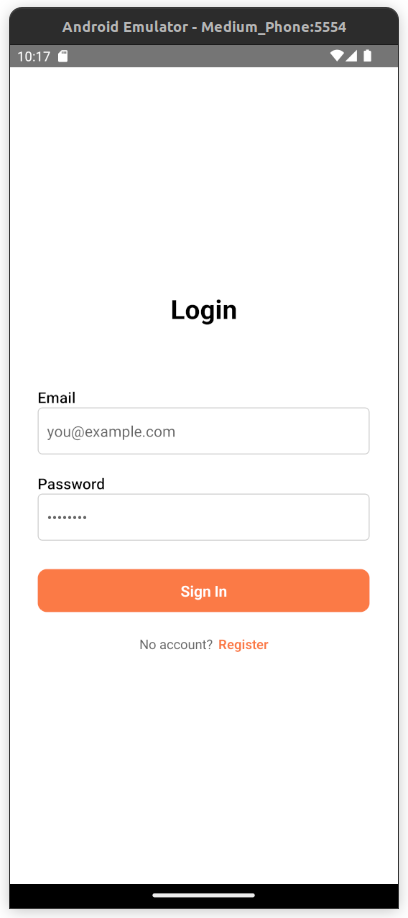
\includegraphics[scale=0.5]{imagenes/LoginScreen}
					\caption{Página de inicio de sesión \hyperref[LoginScreen]{LoginScreen}}
					\label{fig:LoginScreen}
				\end{figure}
			
				%
				%
				%				
				
				\paragraph{Página de registro (RegisterScreen)}
					En el caso de esta página, su función es crear un usuario no existente y para realizar ello, el sistema necesita un correo electrónico y contraseña del usuario.
					El diseño de la página es el siguiente:
					
					\begin{itemize}
						\item Un título mostrando al usuario su posición actual.
						\item Dos campos de texto similares al de la página de inicio de sesión pero en este caso recogen los datos de \textit{email} (correo electrónico) y \textit{password} (contraseña).
						\item Un botón como último componente y que contiene el texto de "registrarse" (\textit{"sign up"} en inglés).
					\end{itemize}
				
					
					\textbf{Lógica de implementación}\\
					La página de registro utiliza una estructura similar a LoginScreen pero orientada a la creación de cuenta:
					
					\begin{itemize}
						\item \textbf{Estado local:} Se gestionan dos estados mediante \texttt{useState}:
						\begin{itemize}
							\item \texttt{email}: almacena el correo del nuevo usuario
							\item \texttt{password}: guarda la contraseña elegida
						\end{itemize}
						
						\item \textbf{Gestión del registro:} La función \texttt{handleRegister} async implementa:
						\begin{itemize}
							\item Validación de campos completos antes de proceder
							\item Limpieza del email con \texttt{trim()}
							\item Llamada a Firebase Auth mediante \texttt{createUserWithEmailAndPassword()}
							\item Manejo de errores con alertas del sistema
						\end{itemize}
						
						\item \textbf{Adaptación multiplataforma:} Al igual que en login, se usa \texttt{KeyboardAvoidingView} para:
						\begin{itemize}
							\item Ajustar la vista cuando aparece el teclado en iOS
							\item Mantener comportamiento nativo en Android
						\end{itemize}
					\end{itemize}
					
					\textbf{Estilos y diseño visual}\\
					Los estilos se mantienen consistentes con LoginScreen mediante \texttt{StyleSheet.create()}:
					
					\begin{itemize}
						\item \textbf{Contenedor:} Usa \texttt{flex: 1} con fondo \texttt{screensBackgroundColor} y padding uniforme
						\item \textbf{Formulario:} Ancho del 90\% y margen superior para separación visual
						\item \textbf{Campos de entrada:} Mantienen el diseño con bordes suaves y espaciado consistente
						\item \textbf{Botón de registro:} Destaca visualmente con el color naranja corporativo y tipografía clara
					\end{itemize}
					
					Esta implementación sigue el principio minimalista mencionado anteriormente, manteniendo solo los elementos esenciales para el registro mientras se asegura una experiencia de usuario fluida y coherente con el resto de la aplicación.
					
					\begin{figure}
						\centering
						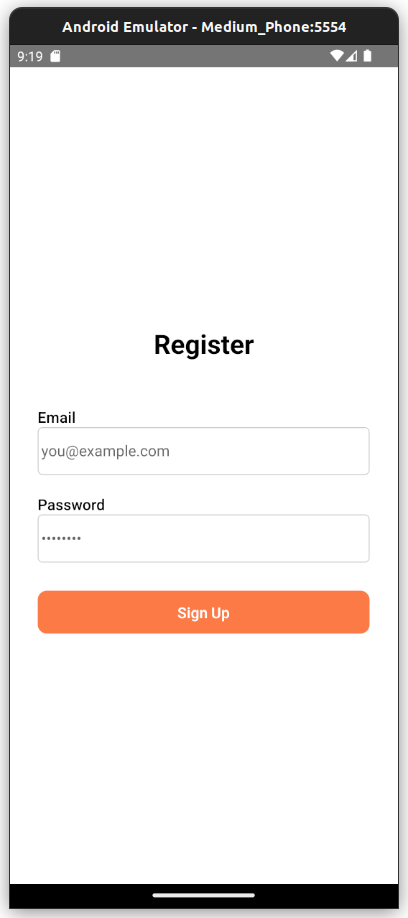
\includegraphics[scale=0.5]{imagenes/RegisterScreen}
						\caption{Página de registro (RegisterScreen)}
						\label{fig:RegisterScreen}
					\end{figure}
					
					En estas dos páginas (\textit{LoginScreen e RegisterScreen}) era posible introducir más componentes, pero dado el principio del minimalismo se decidió mantenerse al menor número de componentes posibles para no sobrecargar las páginas de manera visual y en rendimiento. Por otra parte, no era necesario añadir algo adicional dado que no se requieren datos adicionales.
				
				\paragraph{Página principal (MainScreen)}\label{MainScreen}

					En la planificación del diseño se decidió mostrar el calendario semanal de las recetas planificadas para cada día, pero no era posible mostrar todas las comidas planificadas para toda la semana en una sola pantalla móvil y tampoco era muy minimalista mostrar toda esa información en una sola página; por ello se crearon dos componentes de selección, el primero permite al usuario elegir el día de la semana y el segundo el tipo de comida (desayuno, comida o cena), esto hace que sólo se muestre la lista de una comida de un día específico, simplifica y evita la sobrecarga del diseño de la app.
					La página contiene los componentes en este orden:
					
					\begin{itemize}
						\item Una cabecera que en su izquierda contiene el texto "\textit{Daily Meals}" (comidas diarias) y a su izquierda dos botones uno cierra la sesión y el situado a su derecha abre la página de recetas (\hyperref[RecipesScreen]{RecipesScreen}).
						\item Un menú deslizable horizontalmente que permite al usuario seleccionar el día deseado y que muestra el día seleccionado en naranja.
						\item Otro menú similar al anterior, pero en este caso no es deslizable y sólo tiene la opción de escoger entre desayuno, comida y cena.
						\item Una vista deslizable verticalmente que muestra todos las recetas e ingredientes planificados para el día y comida seleccionados anteriormente.
						\item En la zona inferior derecha hay cuatro botones con diferentes iconos, cada icono muestra la función del botón y estas son.
						\begin{itemize}
							\item Ir a lista de la compra (\textit{GroceryListScreen}).
							\item Ir a la despensa (\textit{PantryScreen}).
							\item Abrir el menú responsable de planificar recetas.
							\item Acceder al menú para añadir nuevas recetas.
						\end{itemize}
					\end{itemize}
					
					\textbf{Lógica de implementación}\\
					La página principal implementa una lógica más compleja que las anteriores debido a su naturaleza central en la aplicación.
					\\
					Esta página tienen varias funciones y procesos que se ejecutan dependiendo de la etapa. Al acceder a \textit{MainScreen} por primera vez (después de haber iniciado sesión) el sistema busca y recoge los ingredientes, recetas y \textit{WeeklyMeals} relevantes para el uso de la aplicación y de mientras muestra un icono de carga. Una vez obtenida la información relevante, se guarda en las variables de \textit{state} de React Native (para permitir futuras actualizaciones) y se muestran en la lista de MainScreen las recetas planificadas del día y el tipo de comida especificado.
					En la zona inferior derecha se encuentran botones de acceso creados para abrir modales para crear o planificar una receta y acceder a las páginas de despensa (\textit{PantryScreen}) y lista de compra (\textit{GroceryListScreen}).
					
					\textbf{Variables y funciones utilizadas}
					\begin{itemize}
						\item \textbf{Estado local:} Gestiona múltiples estados mediante \texttt{useState}:
						\begin{itemize}
							\item \texttt{selectedMeal}: controla el tipo de comida seleccionada
							\item \texttt{selectedDay}: mantiene el día de la semana actual
							\item \texttt{weeklyMeals}: almacena las comidas planificadas
							\item \texttt{currentWeeklyMealsRecipes}: guarda las recetas actuales
							\item \texttt{currentWeeklyMealsIngredients}: mantiene los ingredientes planificados
						\end{itemize}
						
						\item \textbf{Gestión de datos:} Implementa funciones asíncronas para:
						\begin{itemize}
							\item \texttt{fetchWeeklyMeals}: obtiene las comidas planificadas (\textit{WeeklyMeals}) en el día y comida elegidos en los menús superiores.
							\item \texttt{fetchRecipes}: recupera las recetas completas.
							\item \texttt{handlePlanRecipe}: gestiona la planificación de recetas
							\item \texttt{handleUnplanRecipe}: elimina recetas del calendario
						\end{itemize}
						
						\item \textbf{Efectos y ciclo de vida:} Utiliza \texttt{useEffect} para:
						\begin{itemize}
							\item Cargar datos iniciales al montar el componente
							\item Actualizar las comidas cuando cambia el día o tipo de comida
							\item Sincronizar las recetas con las comidas planificadas
						\end{itemize}
					\end{itemize}
					
					\textbf{Estilos y diseño visual}\\
					Los estilos se definen mediante \texttt{StyleSheet.create()} siguiendo un diseño consistente:
					
					\begin{itemize}
						\item \textbf{Contenedor principal:} Utiliza \texttt{flex: 1} con fondo definido en \texttt{screensBackgroundColor}
						\item \textbf{Botones flotantes:} Posicionamiento absoluto con sombras y elevación para efecto visual
						\item \textbf{ScrollView:} Implementado para el desplazamiento vertical suave de las recetas
						\item \textbf{Indicadores de carga:} Centrados y con colores corporativos
					\end{itemize}
					
					Esta implementación sigue un enfoque modular que permite una gestión eficiente de los datos y una experiencia de usuario fluida, manteniendo la consistencia visual con el resto de la aplicación. La separación de responsabilidades entre componentes facilita el mantenimiento y la escalabilidad del código.
					
					\begin{figure}[H]
						\centering
						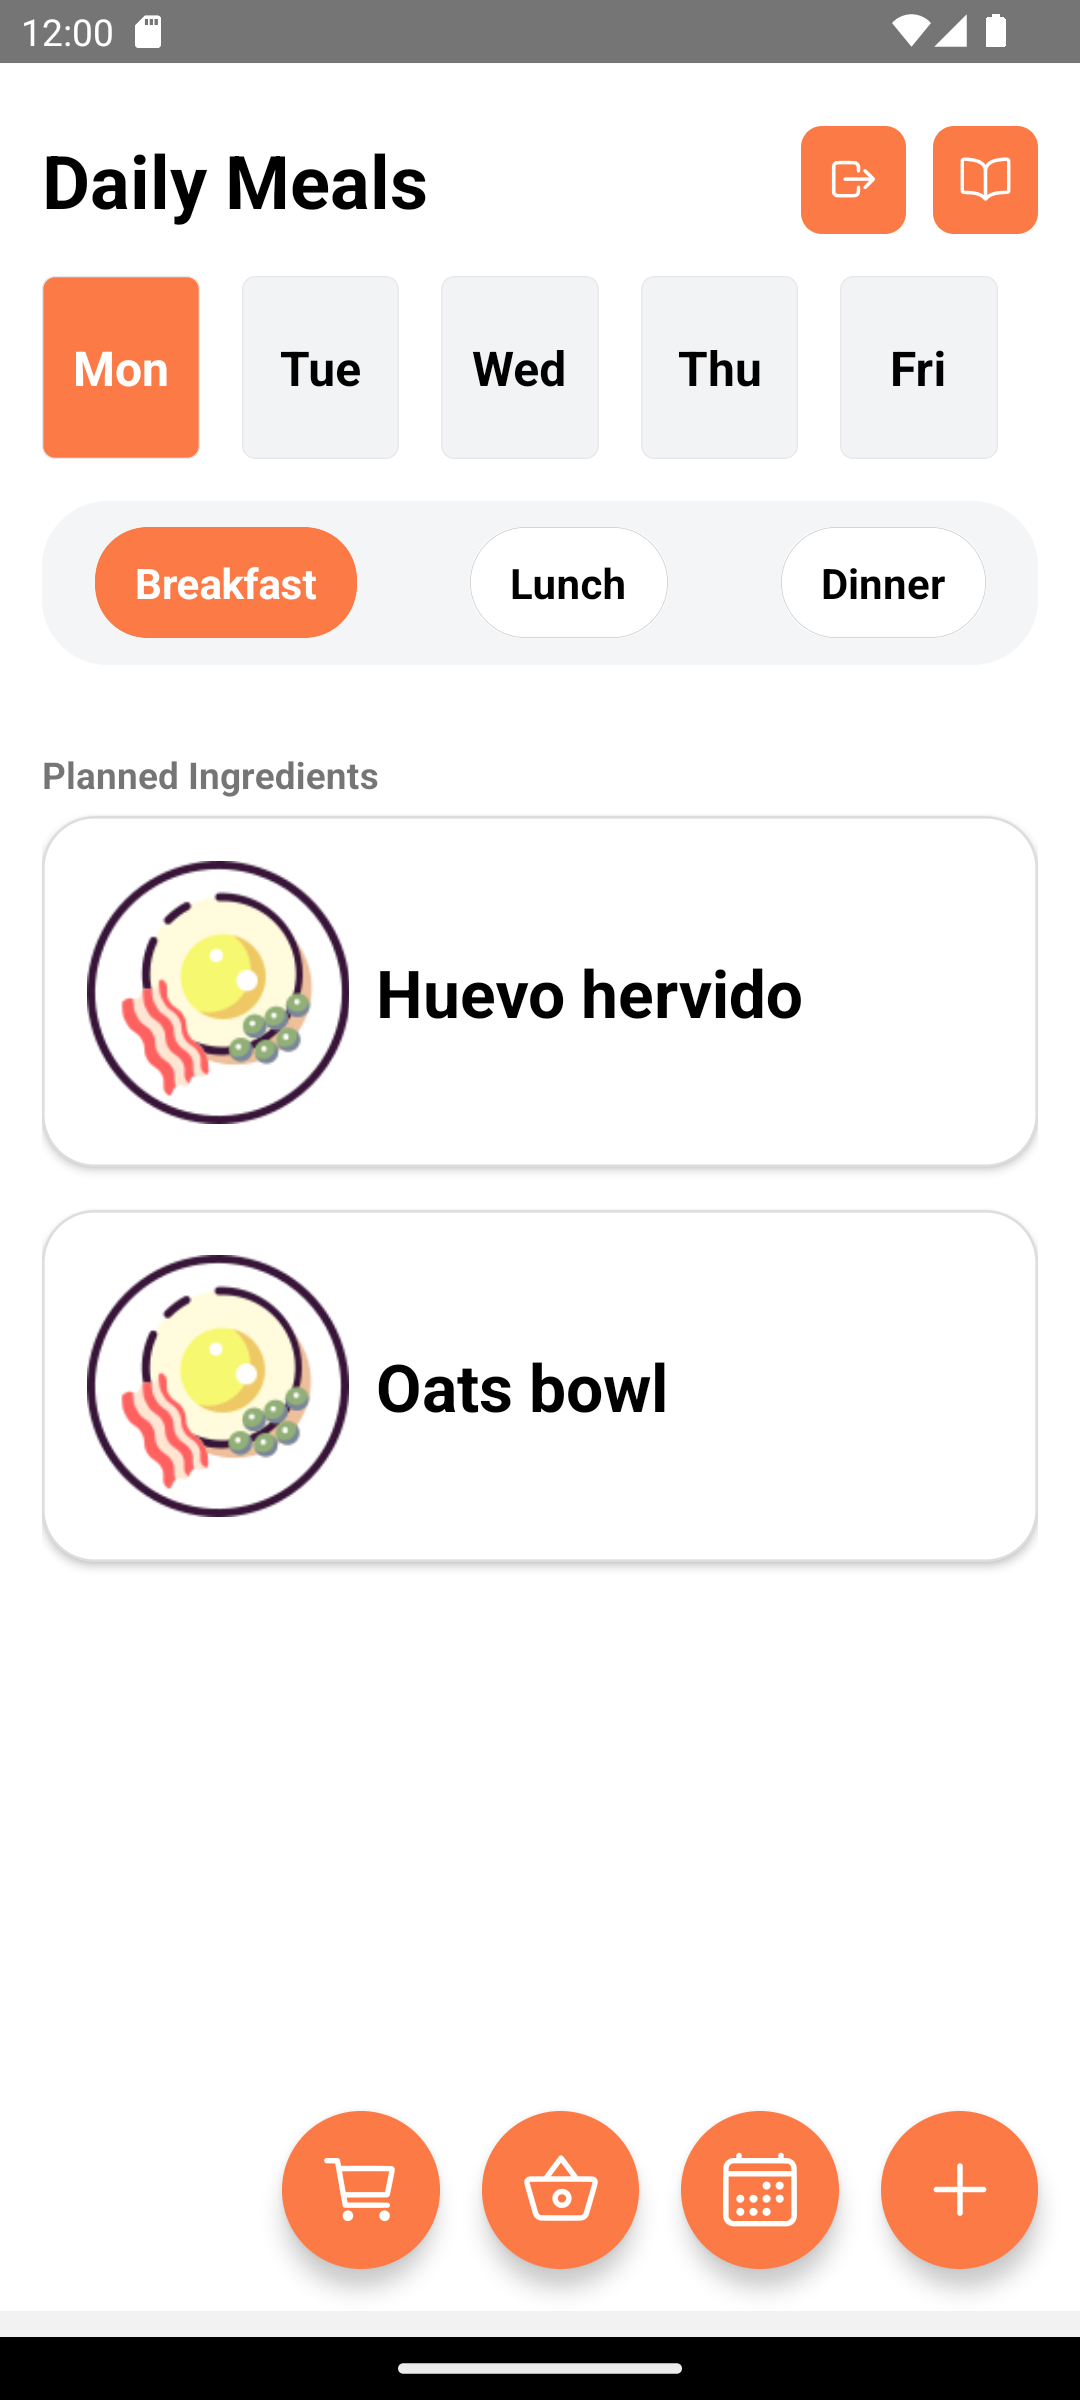
\includegraphics[scale=0.2]{imagenes/MainScreenScreenshot.png}
						\caption{Página principal (MainScreen)}
						\label{fig:MainScreen}
					\end{figure}
			
				%
				%
				%
				
				\paragraph{Página de recetas (RecipesScreen)}
					En esta página se muestran todas las recetas creadas por el usuario. Para mantener el minimalismo y la simplicidad, se ha diseñado de la siguiente manera:
					
					\begin{itemize}
						\item Una cabecera con el texto \textit{Recipes} (Recetas) y un botón de retorno a la página principal.
						\item Una lista deslizable verticalmente que contiene todas las recetas del usuario, cada una representada por un \texttt{RecipeCardComponent} que muestra:
						\begin{itemize}
							\item El título de la receta.
							\item Una imagen si esta existe.
						\end{itemize}
						\item Un botón flotante en la esquina inferior derecha que permite añadir una nueva receta.
					\end{itemize}
					
					Cada tarjeta de receta permite interacción mediante pulsación prolongada, mostrando un menú de opciones para editar o eliminar la receta.
					
					\textbf{Lógica de implementación}\\
					La página de recetas implementa una lógica centrada en la visualización y edición de recetas individuales:
					
					\begin{itemize}
						\item \textbf{Gestión de estado global:} Utiliza el contexto de la aplicación (\texttt{useAppContext}) para acceder y modificar la lista de recetas, permitiendo que los cambios se reflejen en toda la app de manera automática.
						\item \textbf{Navegación:} Emplea el sistema de navegación de React Native para permitir al usuario acceder a la pantalla de detalle de una receta al pulsar sobre una tarjeta, pasando la información relevante como parámetro.
						\item \textbf{Renderizado eficiente:} La lista de recetas se muestra mediante un \texttt{ScrollView}, asegurando un desplazamiento fluido y una experiencia visual agradable incluso con muchas recetas.
						\item \textbf{Interacción con tarjetas:} Cada \texttt{RecipeCardComponent} incluye eventos de pulsación para navegar, y de pulsación prolongada para mostrar opciones adicionales (editar/eliminar), manteniendo la interfaz limpia y funcional.
						\item \textbf{Actualización reactiva:} Al añadir, editar o eliminar una receta, el estado global se actualiza y la lista se re-renderiza automáticamente, garantizando que el usuario siempre vea la información más actual.
					\end{itemize}
					
					\textbf{Estilos y diseño visual}\\
					Los estilos siguen los principios de consistencia y minimalismo presentes en el resto de la aplicación:
					
					\begin{itemize}
						\item \textbf{Contenedor principal:} Fondo definido por \texttt{screensBackgroundColor} y padding uniforme para mantener la coherencia visual.
						\item \textbf{Cabecera:} Espaciado inferior para separar visualmente la cabecera de la lista de recetas.
						\item \textbf{Tarjetas de receta:} Bordes suaves, sombras ligeras y separación entre tarjetas para facilitar la lectura y la interacción.
						\item \textbf{Botón flotante:} Posicionado en la esquina inferior derecha, con color destacado y sombra para resaltar la acción principal de añadir receta.
					\end{itemize}
					
					Esta página mantiene la filosofía de diseño minimalista, mostrando únicamente la información relevante y permitiendo al usuario gestionar sus recetas de forma intuitiva y eficiente.
					
					\begin{figure}[H]
						\centering
						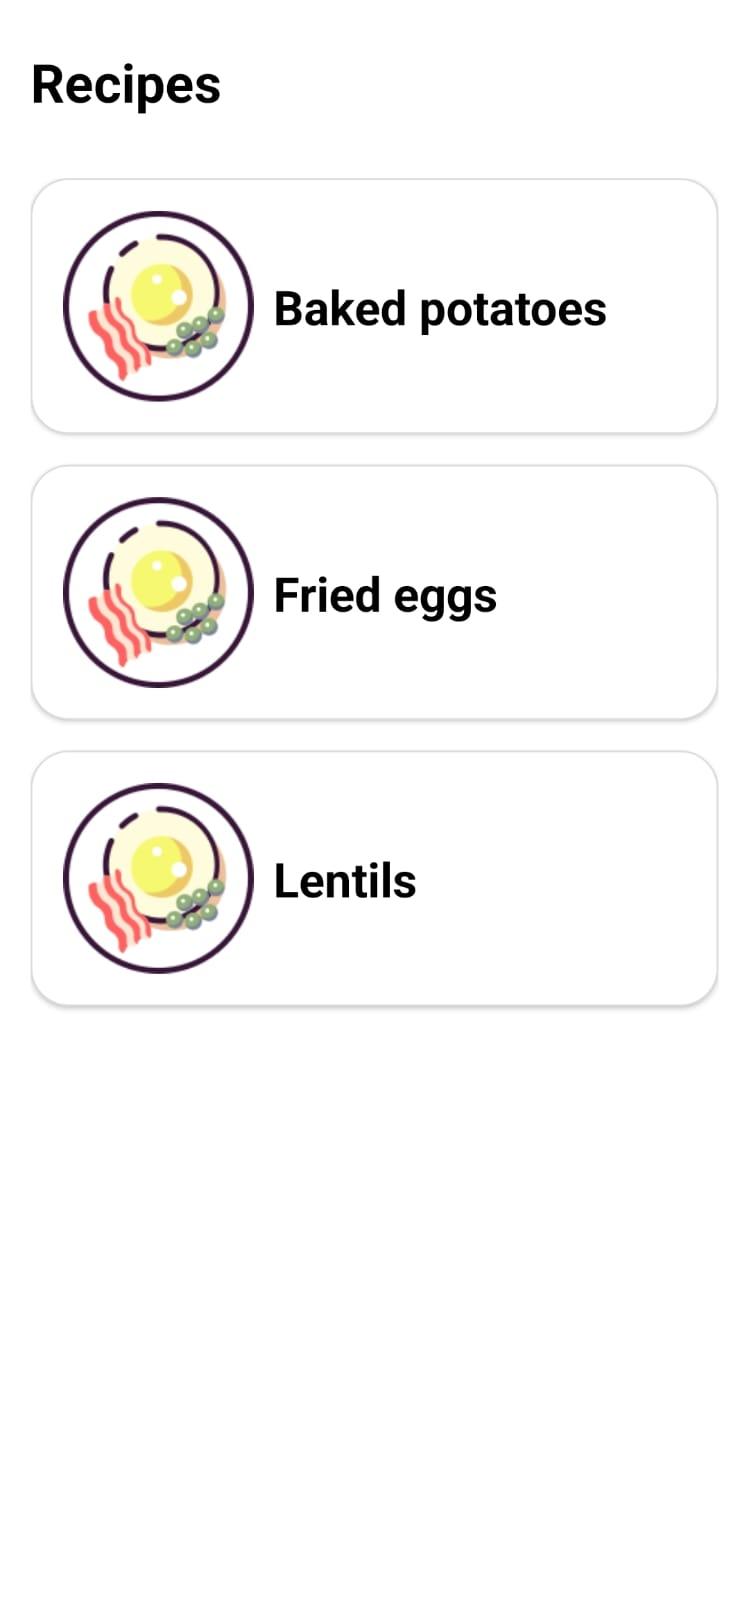
\includegraphics[scale=0.3]{imagenes/RecipesScreen}
						\caption{Página de recetas (RecipesScreen)}
						\label{fig:RecipesScreen}
					\end{figure}

				%
				%
				%
				
				\paragraph{Página de receta individual (RecipeScreen)\\}
				Esta pantalla muestra el detalle completo de una receta específica y permite su edición. Se ha estructurado de la siguiente forma:
				
				\begin{itemize}
					\item Una cabecera con el título de la receta y un botón de retorno.
					\item La imagen de la receta si existe, con un botón para añadir/cambiar imagen.
					\item Una sección de descripción que muestra el detalle de la receta.
					\item Una lista de ingredientes donde cada uno muestra:
					\begin{itemize}
						\item Nombre del ingrediente
						\item Cantidad y unidad de medida
						\item Botón para eliminar el ingrediente
					\end{itemize}
					\item Un botón flotante para añadir nuevos ingredientes a la receta.
				\end{itemize}
				
				\textbf{Lógica de implementación}\\
				La página de receta individual implementa una lógica orientada a la visualización, edición y gestión de los ingredientes de una receta:
				
				\begin{itemize}
					\item \textbf{Gestión de estado local y global:} Utiliza \texttt{useState} para controlar el modo de edición, los cambios realizados y la visibilidad de los modales. El acceso al contexto global (\texttt{useAppContext}) permite modificar la receta y sus ingredientes en toda la aplicación.
					\item \textbf{Edición de receta:} El usuario puede alternar entre modo visualización y edición. En modo edición, los campos de la receta (nombre, enlace, tiempo de preparación, raciones) se muestran como inputs editables. Al guardar, se valida la información y se actualiza el estado global.
					\item \textbf{Gestión de ingredientes:} Los ingredientes se obtienen dinámicamente y se muestran en una lista. En modo edición, cada ingrediente puede modificarse (cantidad, unidad) o eliminarse mediante botones específicos. La adición de ingredientes se realiza a través de un modal de búsqueda y selección.
					\item \textbf{Sincronización y actualización:} Los cambios en los ingredientes o en la receta se sincronizan automáticamente con la base de datos y el estado global, garantizando que la información esté siempre actualizada.
					\item \textbf{Interfaz reactiva:} El diseño permite alternar entre visualización y edición de forma intuitiva, mostrando los botones y campos adecuados según el estado actual.
				\end{itemize}
				
				\textbf{Estilos y diseño visual}\\
				Los estilos mantienen la coherencia con el resto de la aplicación y favorecen la claridad y la usabilidad:
				
				\begin{itemize}
					\item \textbf{Contenedor principal:} Fondo definido por \texttt{screensBackgroundColor} y padding uniforme.
					\item \textbf{Cabecera:} Espaciado inferior y tipografía destacada para el título.
					\item \textbf{Imagen de receta:} Bordes redondeados y tamaño fijo para mantener la estética.
					\item \textbf{Campos de edición:} Inputs con bordes suaves y espaciado consistente.
					\item \textbf{Lista de ingredientes:} Separación clara entre ingredientes, con botones de acción visibles en modo edición.
					\item \textbf{Botón flotante:} Posicionado en la esquina inferior derecha, con color destacado y sombra para resaltar la acción principal de añadir ingrediente.
					\item \textbf{Botón de guardar/editar:} Cambia de icono y texto según el estado, facilitando la interacción.
				\end{itemize}
				
				Esta pantalla permite al usuario consultar y modificar todos los detalles de una receta de forma sencilla y eficiente, manteniendo la filosofía de diseño minimalista y funcional de la aplicación.
				
				\begin{figure}[H]
					\centering
					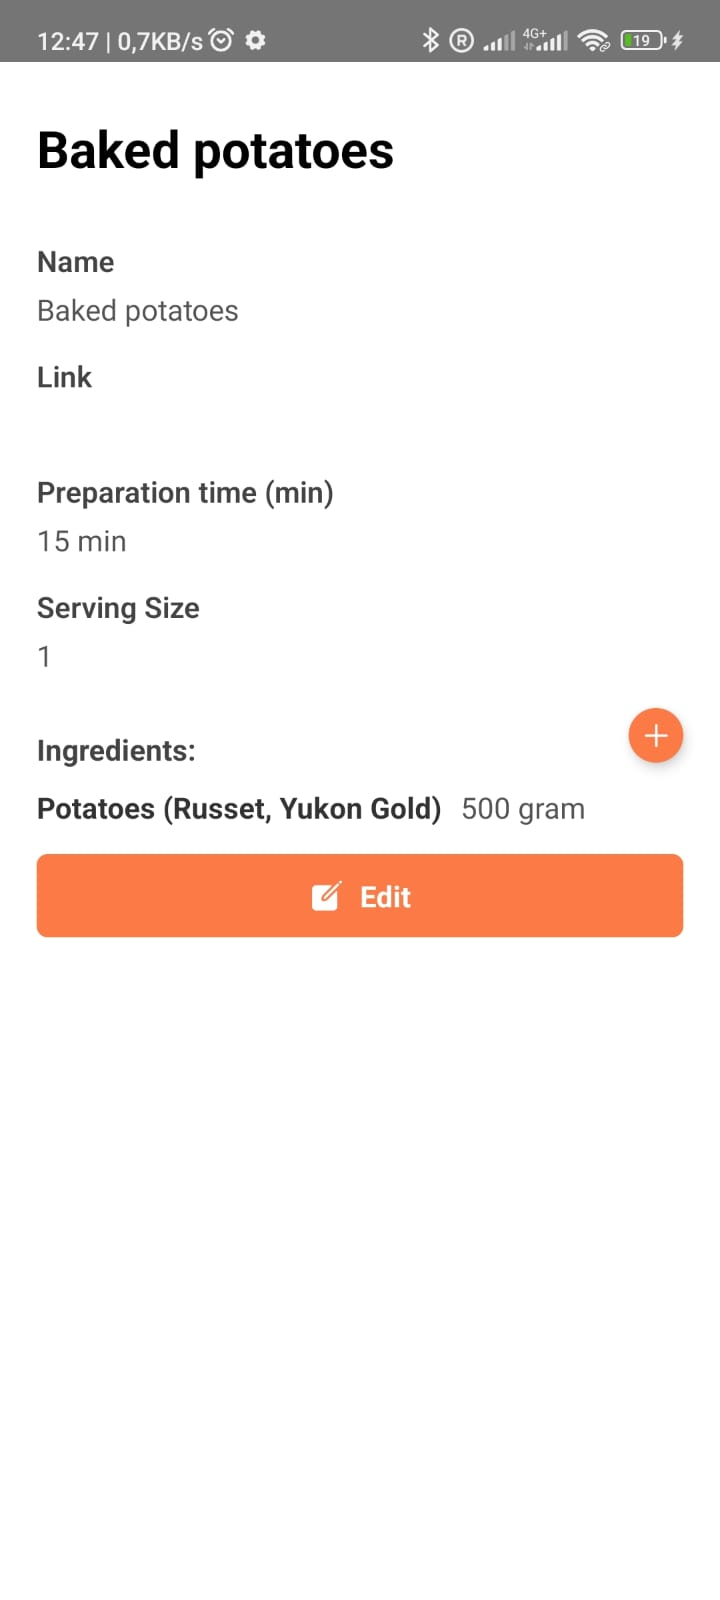
\includegraphics[scale=0.2]{imagenes/RecipeScreen}
					\caption{Página de receta individual (RecipeScreen)}
					\label{fig:RecipeScreen}
				\end{figure}
			
				%
				%
				%
				
				\paragraph{Página de despensa (PantryScreen)}
				La despensa es una parte crucial de la aplicación ya que permite al usuario mantener un registro de los ingredientes disponibles. Su diseño se compone de:
				
				\begin{itemize}
					\item Una cabecera con el texto \textit{Pantry} (Despensa) y botón de retorno.
					\item Una lista deslizable de ingredientes disponibles, donde cada \texttt{IngredientCard} muestra:
					\begin{itemize}
						\item Nombre del ingrediente
						\item Cantidad disponible y unidad
						\item Opción para editar la cantidad
						\item Opción para eliminar el ingrediente de la despensa
					\end{itemize}
					\item Un botón flotante para añadir nuevos ingredientes a la despensa mediante el \texttt{IngredientSearchModal}.
				\end{itemize}
				
				\textbf{Diseño de la lógica}
				La página de la despensa es la encargada de mostrar y permitir al usuario introducir los ingredientes en su despensa. 
				Al abrirse la pantalla, esta muestra el icono de carga para indicar que la app está en proceso de carga y al mismo tiempo pide a la base de datos todos los \textit{PantryIngredients} que este usuario dispone para mostrarlos mediante la función \texttt{getAllIngredientPantries}. Una vez obtenidos se muestran en una lista (ver Figura \ref{fig:PantryScreen}) que permite al usuario ver, cambiar los datos (cantidad, medida) o eliminar el ingrediente.
				Cada vez que el usuario edita añade o elimina un ingrediente la página se encarga de actualizarlo en la base de datos de Firebase.
				
				\begin{figure}[H]
					\centering
					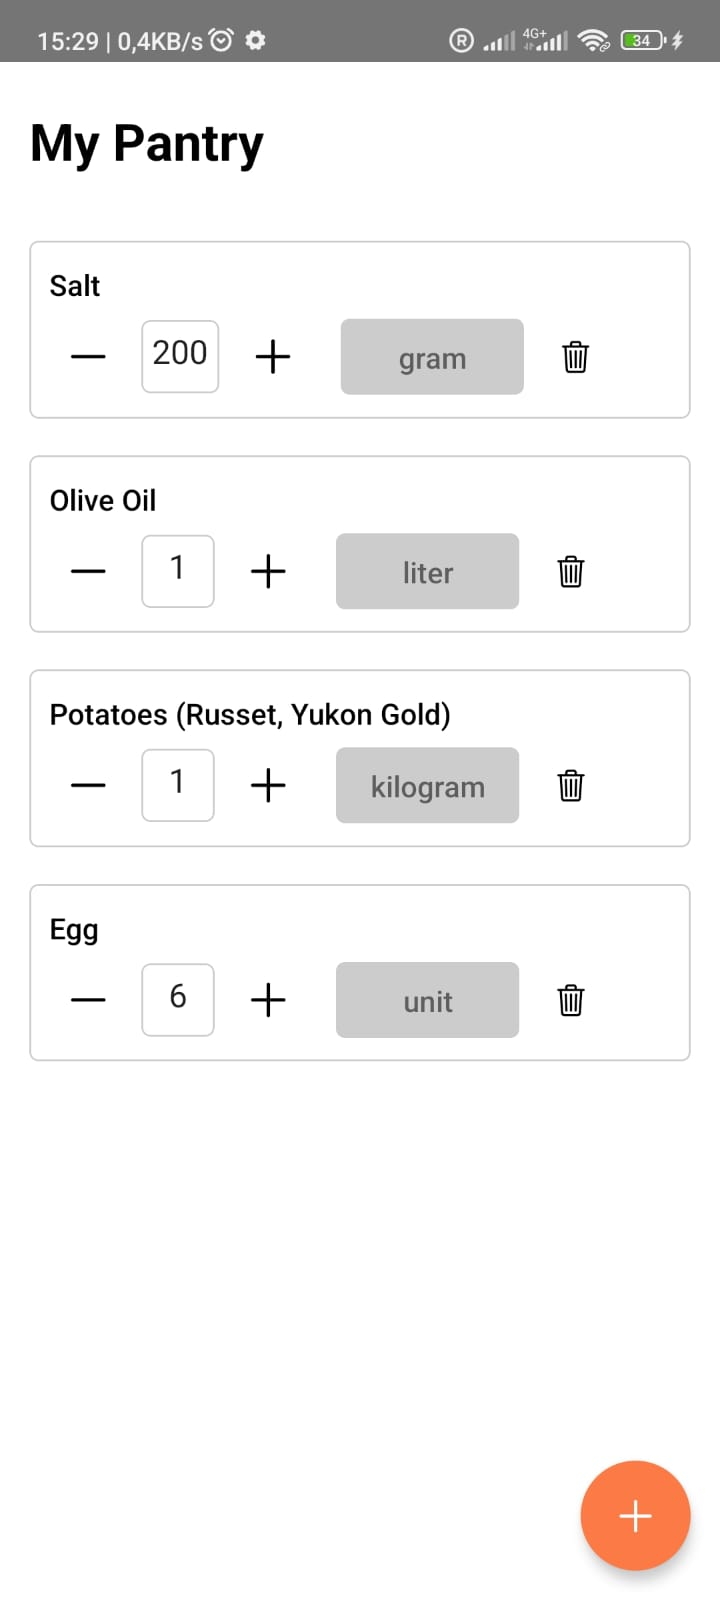
\includegraphics[scale=0.3]{imagenes/PantryScreen}
					\caption{Página de la despensa (PantryScreen)}
					\label{fig:PantryScreen}
				\end{figure}
				
				\paragraph{Página de lista de la compra (GroceryListScreen)}
				Esta página muestra los ingredientes necesarios para las recetas planificadas, calculando automáticamente las cantidades requeridas después de considerar lo disponible en la despensa. Su estructura es:
				
				\begin{itemize}
					\item Una cabecera con el título Grocery List (\textit{Lista de la compra}), un botón de retorno y un botón de actualización que recalcula la lista.
					\item Un texto que muestra la última hora de actualización de la lista.
					\item Una lista deslizable de ingredientes necesarios, donde cada elemento muestra:
					\begin{itemize}
						\item Nombre del ingrediente
						\item Cantidad a comprar y unidad
						\item Un checkbox para marcar como comprado
					\end{itemize}
					\item Una sección colapsable que muestra los ingredientes ya marcados como comprados, permitiendo desmarcarlos si es necesario.
					\item Un mensaje indicando que no hay nada que comprar cuando la lista está vacía.
				\end{itemize}
				
				\textbf{Diseño de la lógica}\\
				Esta página implementa uno de los algoritmos más complejos de la aplicación, ya que debe calcular precisamente qué ingredientes necesita comprar el usuario. El proceso se realiza en varias etapas:
				
				Primero, el sistema recopila todas las comidas planificadas para la semana y las procesa según su tipo. Si es una receta, obtiene todos sus ingredientes; si es un ingrediente individual planificado, lo añade directamente. Durante este proceso, el sistema agrega las cantidades de ingredientes idénticos que comparten la misma unidad de medida. Por ejemplo, si una receta requiere 300g de arroz y otra necesita 200g, estos se combinan en una única entrada de 500g.
				
				Una vez agregados todos los ingredientes necesarios, el sistema consulta el inventario de la despensa del usuario. Para cada ingrediente en la lista de compra, verifica si existe en la despensa y, en caso afirmativo, resta la cantidad disponible de la cantidad necesaria. Por ejemplo, si se necesitan 500g de arroz pero hay 200g en la despensa, la lista de compra mostrará que se deben comprar 300g.
				
				La lista resultante se ordena alfabéticamente y se divide en dos secciones: ingredientes pendientes de comprar e ingredientes ya comprados. Cuando un usuario marca un ingrediente como comprado, este se mueve automáticamente a la sección de comprados y se guarda este estado en la base de datos, permitiendo que la información persista entre sesiones.
				
				El sistema también implementa una actualización en tiempo real: cada vez que se marca o desmarca un ingrediente, o cuando se pulsa el botón de actualizar, se recalcula toda la lista, asegurando que los datos mostrados están siempre sincronizados con el estado actual de la despensa y las comidas planificadas.
				
				\begin{figure}[H]
					\centering
					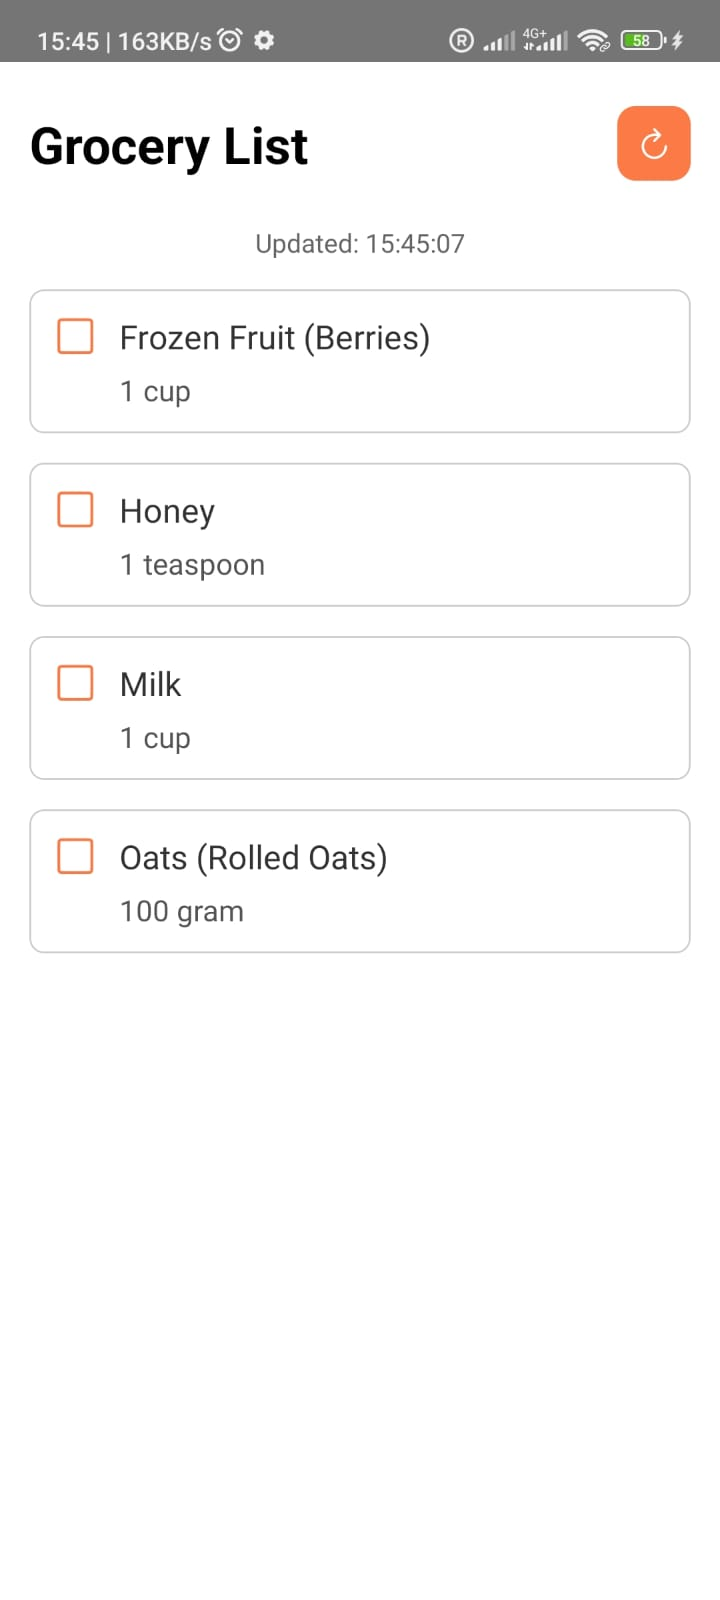
\includegraphics[scale=0.3]{imagenes/GroceryListScreen.jpeg}
					\caption{Página de la lista de la compra (\textit{GroceryListScreen})}
					\label{fig:GroceryListScreen}
				\end{figure}
				
				Esta implementación mantiene el principio de diseño minimalista, mostrando solo la información esencial y manteniendo una jerarquía visual clara. La navegación es intuitiva gracias a los botones de retorno consistentes y el feedback visual inmediato para las acciones del usuario, como el cambio de estado al marcar ingredientes como comprados.
				
				\subsubsection{Flujo de páginas y navegación}
				
				Nuestra aplicación comienza por la página de inicio de sesión (\hyperref[LoginScreen]{LoginScreen} en el caso de no haber iniciado sesión previamente) que tiene acceso a la página de registro (\hyperref[RegisterScreen]{RegisterScreen}) en la que el usuario puede crear una cuenta nueva. Una vez registrado o iniciado sesión, se pasa directamente a la página principal(\hyperref[MainScreen]{MainScreen}) que desde ella se puede acceder a todo el contenido directa e indirectamente, en esta también se muestra la información más relevante y se tiene acceso a \hyperref[RecipesScreen]{RecipesScreen}, \hyperref[PantryScreen]{PantryScreen} y \hyperref[GroceryListScreen]{GroceryListScreen}; se tiene que saber que todas las páginas a las que se accede desde la página principal tienen permitido volver a esta.
				Al mismo tiempo \hyperref[RecipesScreen]{RecipesScreen} que es la página en donde se muestran todas las recetas creadas por el usuario; tiene acceso a \hyperref[RecipeScreen]{RecipeScreen} y esta tiene acceso de vuelta a la página de recetas.
				
				\begin{figure}[H]
					\centering
					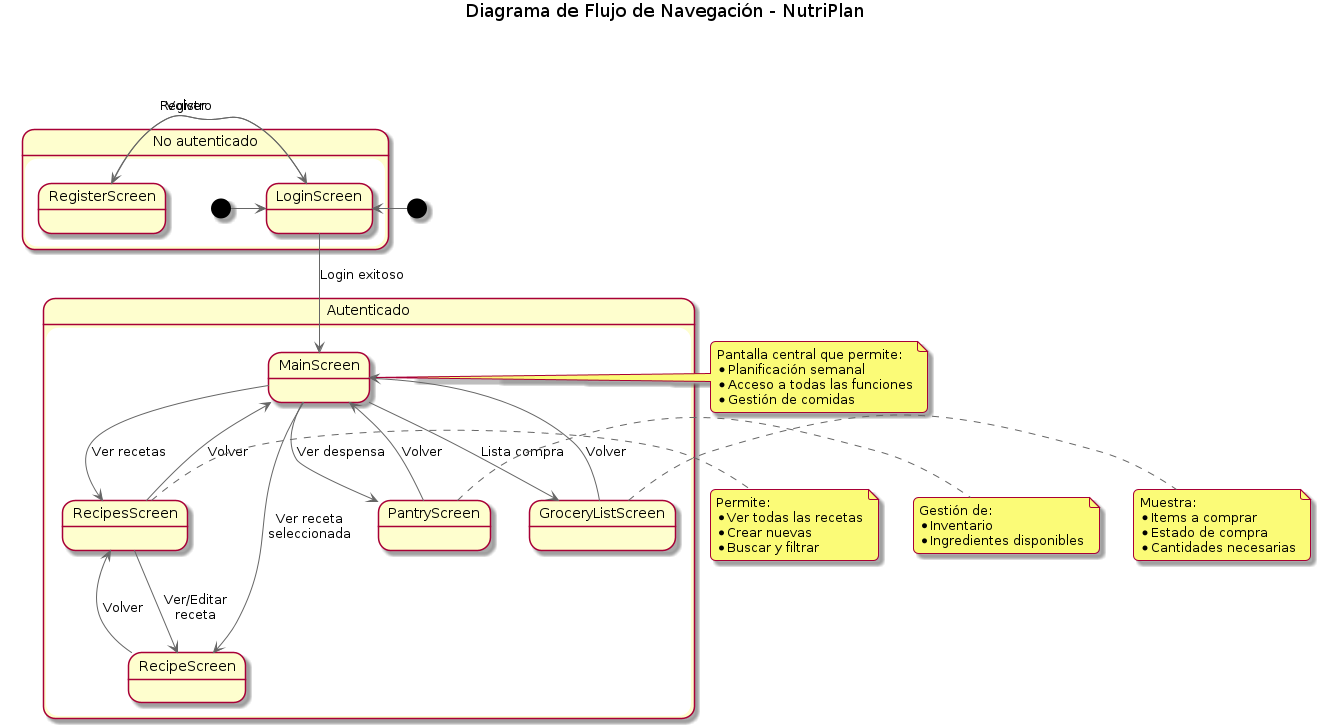
\includegraphics[width=\textwidth]{imagenes/navigation_flow}
					\caption{Diagrama de flujo de navegación de NutriPlan}
					\label{fig:navigation_flow}
				\end{figure}
				
				\paragraph*{Organización y estructura visual}
					La interfaz se organizó priorizando la jerarquía visual y la facilidad de navegación:
					
					\begin{itemize}
						\item \textbf{Barra superior consistente:} Implementada en \texttt{AppHeader}, mantiene el contexto de navegación mostrando títulos en cada sección y provee acceso rápido a funciones y páginas principales. Esta decisión responde al principio de consistencia y reduce la carga cognitiva del usuario al mantener puntos de referencia estables.
						
						\item \textbf{Botones flotantes de acción:} El componente \texttt{FloatingButton} se utiliza para acciones principales (añadir receta, planificar comida) siguiendo patrones de Material Design. Su posición fija en la esquina inferior derecha facilita el acceso con el pulgar, mejorando la ergonomía en uso móvil.
						
						\item \textbf{Tarjetas y listas:} Los componentes \texttt{IngredientCard} y \texttt{RecipeCardComponent} presentan información en bloques visuales claramente delimitados, facilitando el escaneo rápido y la comprensión del contenido.
					\end{itemize}
				
				\paragraph*{Paleta de colores}
					La selección de colores responde tanto a principios de accesibilidad como a la psicología del color en aplicaciones de alimentación:
					
					\begin{itemize}
						\item \textbf{Color primario:} Se eligieron como colores principales el blanco (\#FFF) y el naranja (\#FB7945). El blanco se utiliza principalmente para fondos de pantallas y de componentes; y los colores de las letras. El naranja se utiliza como color de fondo de los componentes(mayoritariamente botones) y también como color para resaltar elementos seleccionados.
						
						\item \textbf{Colores secundarios:} estos también son utilizados frecuentemente y son el gris claro (\#CCC) utilizado para separación sutil entre elementos, color de letras o como fondo de pantalla de otros. Los colores negro y blanco han sido usados para la letra.
						
					\end{itemize}
					
					Esta paleta no solo es estéticamente agradable sino que cumple con ratios de contraste WCAG 2.1 para garantizar accesibilidad.
				
				\paragraph*{Interacción y feedback}
					El diseño de interacciones prioriza la eficiencia y claridad:
					
					\begin{itemize}
						
						\item \textbf{Gestos intuitivos:} Se implementaron gestos naturales como el mantener pulsado en un el \texttt{RecipeCard} para mostrar el modal de opciones
						
						\item \textbf{Feedback visual inmediato:} Cada acción (marcar ingrediente como comprado, añadir a la planificación) tiene una respuesta visual clara que confirma la operación.
					\end{itemize}
				
				\paragraph*{Tipografía y legibilidad}
					Se utilizó una jerarquía tipográfica clara:
					
					\begin{itemize}
						\item \textbf{Títulos:} Fuente System Bold a 20pt para encabezados principales, garantizando visibilidad sin ser intrusiva.
						\item \textbf{Contenido:} System Regular a 16pt para el cuerpo, optimizando legibilidad en pantallas móviles.
						\item \textbf{Información secundaria:} System Light a 14pt para metadatos y detalles adicionales.
					\end{itemize}
				
				\paragraph*{Adaptación a casos de uso}
					El diseño se alineó específicamente con los casos de uso principales:
					
					\begin{itemize}
						\item \textbf{Planificación semanal:} La vista principal (\texttt{MainScreen}) organiza la información por días y comidas, con un selector superior (\texttt{HeaderComponent}) que facilita la navegación temporal.
						
						\item \textbf{Gestión de recetas:} La interfaz de recetas prioriza imágenes y datos clave, permitiendo acceso rápido a ingredientes y cantidades mediante \texttt{IngredientComponent}.
						
						\item \textbf{Lista de compra:} \texttt{GroceryListScreen} implementa una visualización clara de items pendientes vs. comprados, con actualización inmediata del estado.
						
						\item \textbf{Control de despensa:} \texttt{PantryScreen} organiza ingredientes en categorías visuales claras, facilitando el inventario rápido.
					\end{itemize}
				
				\paragraph*{Consideraciones de accesibilidad}
					El diseño incorpora elementos de accesibilidad básicos:
					
					\begin{itemize}
						\item Textos alternativos para imágenes
						\item Áreas táctiles generosas (mínimo 44x44 puntos)
						\item Contraste suficiente entre texto y fondo
						\item Soporte para el escalado de texto del sistema
					\end{itemize}
				
				\paragraph{Iconografía y motivos de elección}
					La iconografía de la aplicación se seleccionó con dos objetivos claros: maximizar la legibilidad y la affordance (que el icono sugiera su acción) y mantener coherencia visual en toda la interfaz. A continuación se recogen los iconos relevantes que aparecen en la aplicación (según la estructura de componentes en \texttt{src/Components}) y la justificación de cada elección.
				
				\paragraph{Librería usada}
					La aplicación emplea una librería de iconos vectoriales (por ejemplo \texttt{react-native-vector-icons} con familias como Ionicons o MaterialCommunityIcons). Esta decisión se fundamenta en su:
					\begin{itemize}
						\item amplia colección de glifos adecuados para interfaces móviles,
						\item escalabilidad y nitidez en pantallas de distinta densidad (vectorial),
						\item facilidad de uso e integración con componentes y temas (color, tamaño, estilos).
					\end{itemize}
				
				\paragraph{Iconos principales y motivos}
					\begin{itemize}
						\item \underline{Añadir / \textit{Plus} (FloatingButton, AddRecipe, AddIngredient).}  
						Se usa el icono de “más” por ser el estándar universal para crear nuevos elementos. Está ubicado en botones flotantes para accesibilidad con el pulgar y destaca con el color primario para indicar la acción principal.
						\item \underline{Buscar / \textit{Search} (IngredientSearchSelector, IngredientSearchModal).}  
						El icono de lupa comunica rápidamente la funcionalidad de búsqueda. Al incluir búsqueda local (MiniSearch) es crítico que el control sea reconocible e inmediato.
						\item \underline{Volver / Flecha atrás (HeaderComponent, navegación).}  
						La flecha dirige la navegación y mantiene la metáfora de pila de pantallas; su colocación consistente en la cabecera reduce la curva de aprendizaje.
						\item \underline{Menú / \textit{Hamburger} o Más opciones (AppHeader, RecipeOptionsModal).}  
						Se utiliza un icono de “más/menú” para agrupar acciones contextuales sin saturar la interfaz principal.
						\item \underline{Editar / \textit{Pencil} (RecipeScreen, ediciones rápidas).}  
						El lápiz es la convención para edición; su uso en modales y tarjetas sugiere edición in‑place en lugar de navegación completa a otra pantalla.
						\item \underline{Eliminar / \textit{Trash} (opciones de receta, lista de compra).}  
						El cubo de basura es inequívoco para borrar elementos; se presenta junto al color de alerta para minimizar acciones accidentales.
						\item \underline{Calendario / Planificación (MainScreen, MealsHeader).}  
						Un icono de calendario o planificación facilita asociar la acción a la gestión temporal (días/turnos) y refuerza la función de plan semanal.
						\item \underline{Carrito de la compra / Grocery (GroceryListScreen).}  
						Icono que remite a compra y lista de la compra; su uso ayuda a distinguir visualmente la vista de compras del inventario.
						\item \underline{Check / Marcar como comprado (GroceryListScreen, PantryScreen).}  
						La marca de verificación indica estado completado/comprado; su reversibilidad en la UI es clave para feedback inmediato.
						\item \underline{Cámara / Imagen (AddRecipeModal).}  
						El icono de cámara sugiere subir o tomar fotos de recetas; refuerza la posibilidad de asociar recursos multimedia a recetas.
						\item \underline{Usuario / Perfil (Login/Register).}  
						El icono de avatar sintetiza las acciones de acceso y perfil; facilita la identificación del flujo de autenticación.
					\end{itemize}
				
				
					
					Las decisiones de diseño tomadas buscan equilibrar simplicidad, eficiencia y satisfacción del usuario, creando una experiencia coherente que facilita la planificación alimentaria y reduce la fricción en tareas cotidianas. La adherencia a principios minimalistas y patrones establecidos de UX móvil contribuye a una curva de aprendizaje suave mientras se mantiene la potencia funcional necesaria.
			
		\subsection{Componentes de la aplicación (Components)}
			\subsubsection{Componentes de la interfaz}
					\paragraph{FloatingButton\\\\}
						\label{FloatingButton}
						
						\textit{Floating Button} (ver Figura \ref{fig:ButtonGroup}) es un botón flotante (componente redondo con sombra) diseñado para acciones primarias en pantalla. El componente ofrece una apariencia de flotación mediante elevación y sombra, y está implementado en \texttt{FloatingButton.tsx} como una función que devuelve el elemento táctil con un icono centrado.\\
						
						\textbf{Descripción funcional\\}
						\begin{itemize}
							\item Botón circular con icono (Ionicons) centrado, pensado para acciones de alto nivel en la interfaz (por ejemplo: añadir, crear, o abrir un modal).
							\item Su posicionamiento por defecto está en la esquina inferior derecha de la pantalla, pero admite estilos personalizados para adaptar posición y apariencia.
							\item La sombra y la elevación proporcionan el efecto visual de estar “flotando” sobre el contenido.
						\end{itemize}
						
						\textbf{Parámetros (props)\\}
						El componente acepta los siguientes parámetros:
						\begin{itemize}
							\item \texttt{onPress: () => void} — función que se ejecuta cuando el botón es pulsado.
							\item \texttt{iconName: IoniconName} — nombre del icono a mostrar (válido dentro de las opciones de Ionicons).
							\item \texttt{iconColor?: string} — color del icono (opcional; por defecto \texttt{'white'}).
							\item \texttt{iconSize?: number} — tamaño del icono en dp (opcional; por defecto \texttt{28}).
							\item \texttt{containerStyle?: ViewStyle} — estilos adicionales para el contenedor del botón (opcional; permite sobrescribir posición, tamaño, color, etc.).
							\item \texttt{iconContainerStyle?: ViewStyle} — estilos adicionales aplicables al icono (opcional).
						\end{itemize}
						
						\textbf{Contrato y comportamiento\\}
						\begin{itemize}
							\item Entrada: las props indicadas y la interacción del usuario (tap).
							\item Salida: invocación de \texttt{onPress} cuando el usuario pulsa el botón; no realiza otras mutaciones ni llamadas internas por defecto.
							\item Comportamiento por defecto: si no se proporcionan estilos, el botón se muestra en la esquina inferior derecha con fondo de color de acento, tamaño fijo (60×60) y borde redondeado completo.
							\item Extensibilidad: mediante \texttt{containerStyle} y \texttt{iconContainerStyle} es posible adaptar posición, tamaño y apariencia sin modificar la lógica interna.
						\end{itemize}
						
						\begin{figure}[H]
							\centering
							
\includegraphics{imagenes/ButtonGroup}
							\caption{\textit{FloatingButton} — ejemplo de botón flotante}
							\label{fig:ButtonGroup}
						\end{figure}
					
					%
					%
					%
					
					\paragraph{IngredientCard\\\\}
					\label{subsec:ingredientcard}
					
					El componente \texttt{IngredientCard} (ver Figura \ref{fig:IngredientCard}) es una tarjeta de presentación de datos cuyo propósito es mostrar sin permitir su modificación la información relevante de un \texttt{RecipeIngredient} asociado a una receta. Está concebido como un componente puramente presentacional que recibe un único parámetro con la estructura del ingrediente (identificador, nombre, cantidad y unidad) y lo renderiza de forma clara para el usuario. Se utiliza en la página \hyperref[RecipeScreen]{RecipeScreen} y en el modal \hyperref[AddRecipeModal]{AddRecipeModal} como elemento de la lista de ingredientes de una receta.

					
					\textbf{\\Parámetros y contrato\\}
					\begin{itemize}
						\item \underline{Prop principal:} un objeto de tipo \texttt{RecipeIngredient} (o similar) que contiene al menos \texttt{id}, \texttt{name}, \texttt{quantity} y \texttt{quantityType}.
						
						\item \underline{Contrato:} entrada = datos de un \texttt{RecipeIngredient}; salida = renderizado visual; efectos secundarios = ninguno. El componente garantiza no mutar los datos recibidos y no invocar callbacks de modificación.
						
						\item \underline{Precondiciones:} el objeto recibido debe contener un identificador único y un nombre legible; la cantidad puede ser numérica o nula (el componente debe mostrar \texttt{N/A} o un marcador equivalente cuando falten datos).
					\end{itemize}
					
					\textbf{Comportamiento y flujo\\}
					\begin{itemize}
						\item Al recibir un \texttt{RecipeIngredient}, renderiza en orden: título/etiqueta, nombre del ingrediente y la línea de cantidad/unidad.
						\item Si faltan campos (por ejemplo, \texttt{quantityType}), muestra un indicador textual coherente (por ejemplo, \texttt{N/A}).
						\item Diseñado para ser usado en listados; se recomienda emplear como \texttt{key} en mapeos el \texttt{id} del \texttt{RecipeIngredient} para evitar re-renderizados innecesarios.
					\end{itemize}
					
					\textbf{Ejemplo de uso\\}
					A modo ilustrativo, en \texttt{RecipeScreen} o \texttt{AddRecipeModal} se utiliza típicamente dentro de un mapeo:
					
					\begin{lstlisting}[language=TypeScript]
						// Fragmento de ejemplo
						import { IngredientCard } from '../Components/IngredientCard';
						
						// dentro del render
						{recipeIngredients.map(ri => (
							<IngredientCard key={ri.id} recipeIngredient={ri} />
							))}
					\end{lstlisting}
					
					\begin{figure}[H]
						\centering
						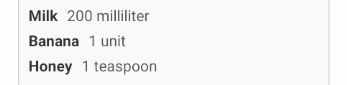
\includegraphics{imagenes/IngredientCard}
						\caption{Ejemplos del componente \textit{IngredientCard}}
						\label{fig:IngredientCard}
					\end{figure}
				
					%
					%
					%
					
					\paragraph{AppHeader\\\\}
					
					\label{AppHeader}
					
					El componente \texttt{AppHeader} (ver Figura \ref{fig:AppHeader}) se utiliza para mostrar las cabeceras en las distintas pantallas de la aplicación. Está diseñado como un componente funcional que recibe un texto para mostrar como título y, opcionalmente, un componente que se situará a la derecha del título (por ejemplo, un botón de acción o un icono). Su objetivo es proporcionar una presentación consistente en las cabeceras de las páginas y facilitar la reutilización en todas las vistas. 
					
					\textbf{\\Parámetros\\}
					
					\begin{itemize}
						\item \texttt{title: string} — cadena que contiene el texto a mostrar en la cabecera.
						\item \texttt{rightComponent?: React.ReactNode} — componente opcional que se renderiza a la derecha del título.
					\end{itemize}
					
					\begin{figure}[H]
						\centering
						
\includegraphics{imagenes/AppHeader}
						\caption{\textit{AppHeader}}
						\label{fig:AppHeader}
					\end{figure}
					
					%
					%
					%
					
					\paragraph{HeaderComponent\\\\}
					\label{HeaderComponent}
					
					El componente \texttt{HeaderComponent} (ver en Figura \ref{fig:HeaderComponent}) se utiliza como cabecera específica de la pantalla principal (\hyperref[MainScreen]{\texttt{MainScreen}}). Está compuesto por una cabecera superior reutilizable (\texttt{\hyperref[AppHeader]{AppHeader}}) y una vista deslizable horizontal que presenta los días de la semana para permitir al usuario seleccionar el día deseado (\texttt{\hyperref[MealTypeComponent]{MealTypeComponent}}). Su propósito es ofrecer una navegación rápida entre los días y mantener coherencia visual con el resto de la interfaz.\\
					
					\textbf{Contrato:\\}
					\begin{itemize}
						\item Entrada: el día seleccionado actual, la función que lo modifica y la acción a ejecutar al pulsar el botón derecho.
						\item Salida: invocaciones a \texttt{setSelectedDay} cuando el usuario selecciona un día, y a \texttt{onButtonPress} al pulsar el botón auxiliar.
						\item Efectos secundarios: ninguno persistente; la mutación del estado se realiza en el contenedor mediante las funciones pasadas.
					\end{itemize}
					
					\textbf{Comportamiento de interacción\\}
					\begin{itemize}
						\item Al tocar una tarjeta de día se ejecuta \texttt{setSelectedDay(day)}, provocando que la tarjeta pase a estado activo (cambio de color de fondo y texto).
						\item El botón ubicado en la parte superior derecha delega su acción a \texttt{onButtonPress}, permitiendo al contenedor decidir la operación (por ejemplo, navegar a otra pantalla o abrir un modal).
						\item La vista deslizable admite desplazamiento horizontal y oculta el indicador de scroll para una presentación limpia.
					\end{itemize}
					
					\begin{figure}[H]
						\centering
						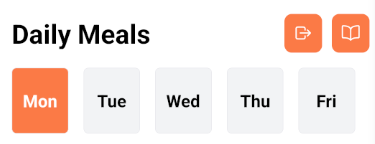
\includegraphics{imagenes/HeaderComponent}
						\caption{\textit{HeaderComponent} debajo de \textit{AppHeader}}
						\label{fig:HeaderComponent}
					\end{figure}
				
				%
				%
				%
				
				\paragraph{IngredientComponent\\\\}
				\label{IngredientComponent}
				
				Este componente es una unidad de interfaz que recibe como entrada un objeto  \texttt{RecipeIngredient} (identificado por su \texttt{id}) junto con callbacks para actualizar cantidad, tipo de unidad y para eliminar el ingrediente. Su responsabilidad es presentar el nombre, la cantidad y la métrica del ingrediente y ofrecer controles de interacción (botones y campo numérico) que delegan la lógica de mutación en el componente contenedor.
				
				\textbf{\\Interfaz (props) y contrato\\}
				El componente acepta las siguientes props (tipado en TypeScript, tal y como aparece en el código):
				\begin{itemize}
					\item \texttt{ingredients: Ingredient[]} — lista completa de ingredientes disponibles (usada para identificar el nombre por \texttt{id}).
					\item \texttt{id: string} — identificador único del ingrediente que este componente representa.
					\item \texttt{quantity: number} — cantidad actual asignada.
					\item \texttt{quantityType: QuantityType} — tipo de unidad asociado a la cantidad (p. ej. GRAM, ML, UNIT).
					\item \texttt{number: number} — índice/posición del componente en la lista (empleado únicamente para estilos como \texttt{zIndex}).
					\item \texttt{setQuantity: (quantity: number) => void} — callback para actualizar la cantidad (la mutación real la realiza el contenedor).
					\item \texttt{setQuantityType: (quantityType: QuantityType) => void} — callback para actualizar la unidad.
					\item \texttt{onDelete: (id: string) => void} — callback para eliminar el ingrediente por su \texttt{id}.
				\end{itemize}
				
				\textbf{Contrato:}
				\begin{itemize}
					\item Entrada: props listadas arriba y la interacción del usuario (teclado, botones).
					\item Salida: invocaciones a \texttt{setQuantity}, \texttt{setQuantityType} y \texttt{onDelete} con los parámetros esperados.
				\end{itemize}
				
				\begin{figure}[H]
					\centering
					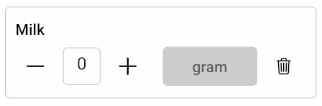
\includegraphics{imagenes/IngredientComponent}
					\caption{\textit{IngredientComponent}}
					\label{fig:IngredientComponent}
				\end{figure}
				
				%
				%
				%
				
				
					
			\subsubsection{Componentes modales}
				\paragraph{AddIngredientModal\\\\}
					\label{AddIngredientModal} 
					%
					AddIngredientModal ver Figura \ref{fig:AddIngredientModal}. Modal encargado de añadir ingredientes en la base de datos. Contiene dos campos de texto para insertar el nombre y la categoría del ingrediente y tres botones, uno superior encargado de cerrar el modal y dos inferiores, uno cancela el proceso (botón "\textit{cancel}") y otro (botón "\textit{Add Ingredient}") que al ser pulsado confirma que los datos insertados sean correctos, el nuevo ingrediente no exista en la base de datos para finalmente añadir el ingrediente, mostrar un mensaje de confirmación al usuario y cerrar el modal.
						
					\begin{figure}[H]
						\centering
						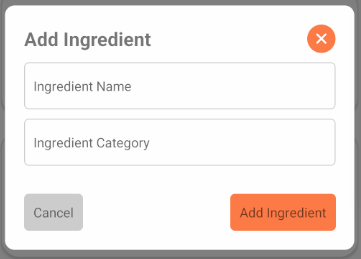
\includegraphics{imagenes/AddIngredientModal}
						\caption{Modal de \textit{AddIngredient}}
						\label{fig:AddIngredientModal}
					\end{figure}
				\paragraph{AddRecipeModal\\\\}\label{AddRecipeModal}
					AddRecipeModal (Ver Figura \ref{fig:AddRecipeModalPrimeraParte}). Es mostrado cuando el usuario pulsa en el botón de añadir receta situado en la parte inferior de  \hyperref[MainScreen]{MainScreen}, está formado por tres secciones, la primera es la encargada de crear la colección \hyperref[Recipe]{Recipe} (Receta), contiene un botón de selección de imagen, cuatro campos de texto (para el nombre, enlace, tiempo de preparación y raciones) y un botón para pasar a la siguiente fase. Esta sección no permite al usuario pasar a la siguiente si no se han rellenado los datos necesarios. 
						
						\begin{figure}[H]
							\centering
							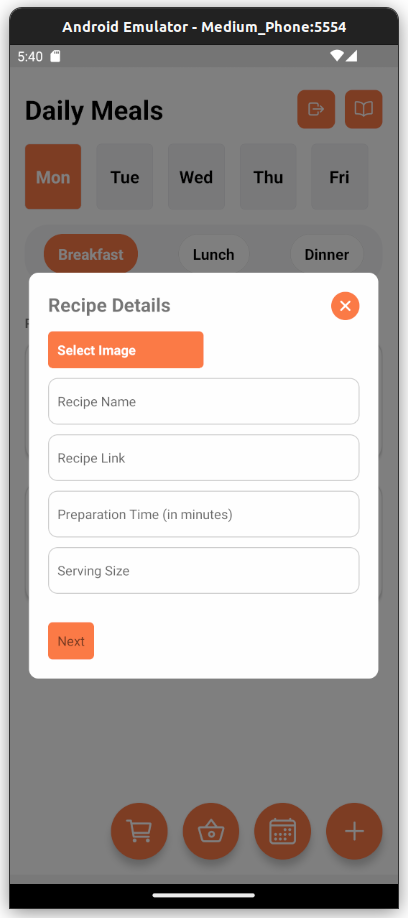
\includegraphics{imagenes/AddRecipeModal}
							\caption{Primera sección del \textit{AddRecipe} Modal}
							\label{fig:AddRecipeModalPrimeraParte}
						\end{figure}
						
					La segunda sección (ver Figure \ref{fig:AddRecipeModalSegundaParte}) es la encargada de permitir al usuario escoger todos los ingredientes necesarios para esta receta, añadir sus cantidades y confirmar que estas sean correctas. Consiste de una barra de búsqueda (\hyperref[IngredientSearchModal]{IngredientSearchModal}) que facilita al usuario encontrar un ingrediente determinado; en el caso de no encontrarlo, existe un botón a su derecha que abre el modal que crea un ingrediente (\textit{\hyperref[AddRecipeModal]{AddRecipeModal}}); debajo de ellos se encuentra una vista desplazable(\textit{ScrollView}) que contiene la lista de los ingredientes que el usuario va escogiendo y que permite a este desplazarse verticalmente entre ellos. Los ingredientes escogidos son mostrados en la lista usando el componente \hyperref[IngredientComponent]{\textit{IngredientComponent}} que permite visualizar, modificar o eliminar las cantidades del ingrediente escogido, seguido de un botón que comprueba que las cantidades de los ingredientes son correctas y lleva a la última sección; y otro botón que devuelve al usuario a la primera sección.
							
					\begin{figure}[H]
						\centering
						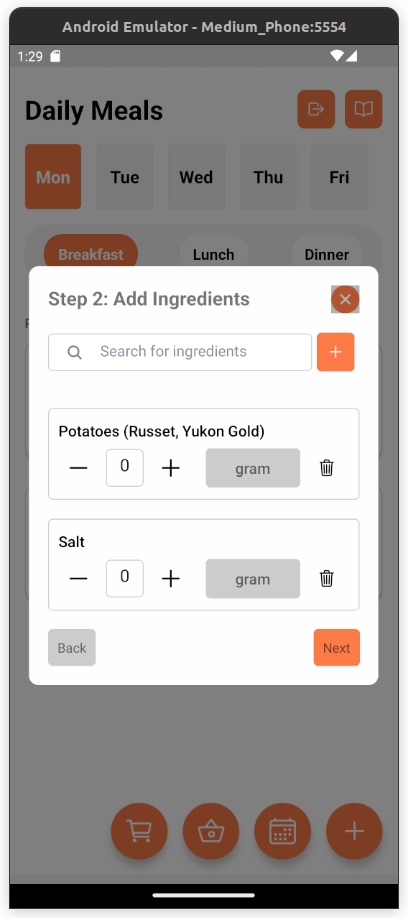
\includegraphics[]{imagenes/AddRecipeModalSegundaParte}
						\caption{Segunda sección de \textit{AddRecipe} Modal (selección de RecipeIngredients)}
						\label{fig:AddRecipeModalSegundaParte}
					\end{figure}
							
					En la tercera y última sección, se muestran todos los datos e ingredientes introducidos en las secciones anteriores para que el usuario las compruebe y confirme la adición de la receta en la aplicación. La confirmación se realiza al pulsar en el botón de "\textit{Save Recipe} (Guardar receta)", esto hace que el sistema recoja todos los datos, cree la receta, los \textit{RecipeIngredients} (Ingredientes de la receta) y añade estos en la base de datos. Una vez finalizados los procesos muestra un mensaje de confirmación al usuario y la receta es mostrada en la pantalla de recetas (\textit{RecipeScreen})
							
					\begin{figure}[H]
						\centering
						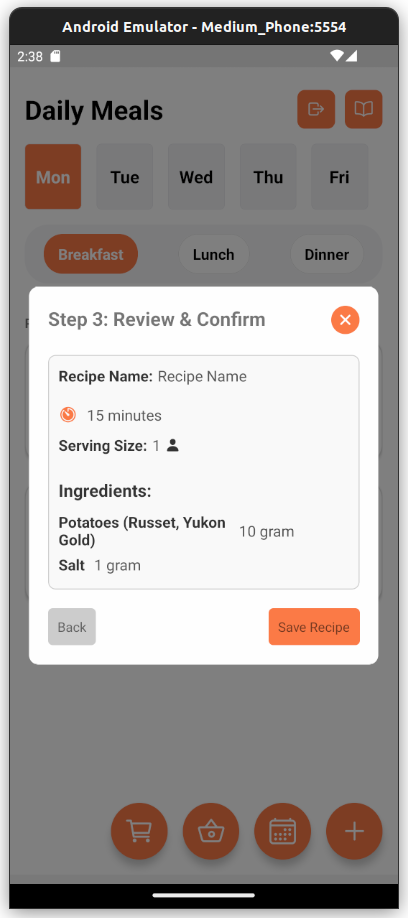
\includegraphics{imagenes/AddRecipeModalTerceraParte}
						\caption{Tercera sección de \textit{Addrecipe} Modal}
						\label{fig:AddRecipeModalTerceraParte}
					\end{figure}

				\paragraph{IngredientSearchModal\\\\} \label{IngredientSearchModal}
					Este modal es la herramienta principal para buscar y seleccionar ingredientes existentes o añadir uno nuevo cuando no se encuentra. Se presenta como una ventana emergente con una barra de búsqueda en la parte superior que indexa los ingredientes locales usando MiniSearch, mostrando resultados en tiempo real. Este modal está pensado para ser rápido, tolerante a entradas parciales y funcionar sin dependencia de la red, por lo que la experiencia es fluida incluso en condiciones de conectividad limitada. A nivel de interacción, el modal ofrece un flujo corto: búsqueda, selección y confirmación; si el usuario no encuentra el ingrediente, dispone de un acceso directo al modal de creación de ingrediente.
					
					\begin{figure}[H]
						\centering
						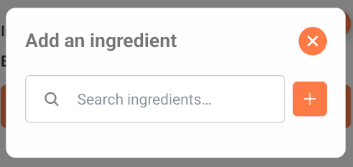
\includegraphics{imagenes/IngredientSearchModal}
						\caption{\textit{IngredientSearch} modal}
						\label{fig:IngredientSearchModal}
					\end{figure}

				\paragraph{IngredientSearchSelectorComponent\\\\}
					Es una versión compacta y reutilizable del selector de ingredientes usado dentro de otros modales y pantallas. Su propósito es encapsular la lógica de búsqueda, selección múltiple y visualización de las entradas seleccionadas en una forma que pueda integrarse dentro de otros formularios sin duplicar código. Desde el punto de vista del diseño, su comportamiento prioriza la claridad: muestra las coincidencias, permite seleccionar una entrada y ajustar su cantidad, y comunica los cambios al contenedor mediante callbacks. Esta separación facilita mantener la lógica de búsqueda aislada y reutilizable en diferentes contextos de la aplicación.
					
					

				\paragraph{CustomPicker\\\\}
					El \texttt{CustomPicker} es un selector personalizado que sustituye a pickers nativos para ofrecer un aspecto y comportamiento homogéneo entre plataformas. Se utiliza principalmente para escoger el \texttt{quantityType} (unidad de medida) en los componentes que requieren selección de unidades. Está implementado como un modal ligero que muestra una lista de opciones con feedback táctil y permite cerrar la selección sin cambiar el valor. Este componente asegura consistencia visual y evita diferencias de comportamiento entre iOS y Android.
						
					\begin{figure}[H]
						\centering
						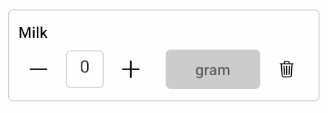
\includegraphics{imagenes/CustomPicker.png}
						\caption{\textit{CustomPicker}}
						\label{fig:CustomPicker}
					\end{figure}
					
					\begin{figure}[H]
						\centering
						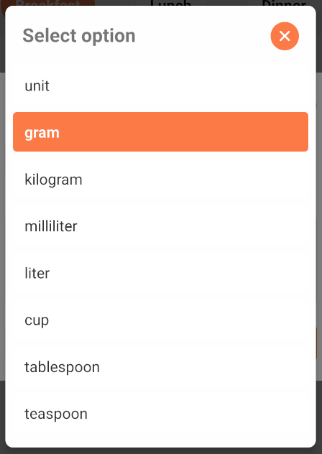
\includegraphics{imagenes/CustomPickerModal}
						\caption{\textit{CustomPickerModal}}
						\label{fig:CustomPickerModal}
					\end{figure}

				\paragraph{AddIngredientButton\\\\}
					El pequeño componente \texttt{AddIngredientButton} actúa como disparador de la creación rápida de ingredientes desde contextos donde el usuario está añadiendo recetas o editando la despensa. Su diseño es compacto y reconocible (icono +) y su responsabilidad es abrir el modal de creación de ingrediente (\hyperref[AddIngredientModal]{AddIngredientModal}), centralizando la lógica de navegación y manteniendo la UI limpia. Su existencia evita repetir el mismo control en múltiples lugares y mejora la coherencia de la interfaz.
						
					\begin{figure}[H]
						\centering
						
\includegraphics{imagenes/AddIngredientButton.png}
						\caption{\textit{AddIngredientButton} modal}
						\label{fig:AddIngredientButton}
					\end{figure}

				\paragraph{MealsHeader\\\\}
					\texttt{MealsHeader} (ver figura \ref{fig:HeaderComponent}) es un componente de cabecera específico para la pantalla de planificación semanal. Combina elementos de navegación temporal (selección de día) con controles de contexto (tipo de comida), organizando la información de forma que el usuario pueda cambiar rápidamente el día o la comida a la que desea asignar recetas. Está diseñado para ser compacto y semántico: el día y el tipo de comida son los ejes que determinan el contenido mostrado en la pantalla principal.
						

				\paragraph{MealTypeComponent\\\\} \label{MealTypeComponent}
				El \texttt{MealTypeComponent} abstrae la selección del tipo de comida (desayuno, comida, cena). Presenta botones o fichas con el nombre de la comida y resalta la opción activa. Su mérito principal es separar la lógica de presentación del tipo de comida del resto de la pantalla, facilitando usar la misma pieza en diferentes vistas y simplificando pruebas y mantenimiento.
						
					\begin{figure}[H]
						\centering
						
\includegraphics{imagenes/MealPicker.png}
						\caption{\textit{AddIngredientButton} modal}
						\label{fig:MealType}
					\end{figure}

				\paragraph{ModalHeaderComponent\\}
					El componente \texttt{ModalHeaderComponent} actúa como cabecera reutilizable dentro de los modales complejos. Provee el título, el botón de cierre y, opcionalmente, atajos contextuales (por ejemplo, guardar o retroceder). Su uso mejora la coherencia entre los distintos modales y reduce la repetición de código para la gestión de la zona superior de estas ventanas. Este es usado en varios modales como \textit{IngredientSearchModal} (ver la cabecera del componente en la figura \ref{fig:IngredientSearchModal}).
						

				\paragraph{PlannedIngredientCard}
					\texttt{PlannedIngredientCard} es la representación compacta de un ingrediente incluido en la planificación semanal. A diferencia de \texttt{IngredientCard}, incluye información sobre el contexto de planificación (día, comida) y permite acciones rápidas como desasignar o ajustar la cantidad propuesta. Su papel es servir de elemento visual en listados de planificación, manteniendo un equilibrio entre detalle y compacidad.
						
					\begin{figure}[H]
						\centering
						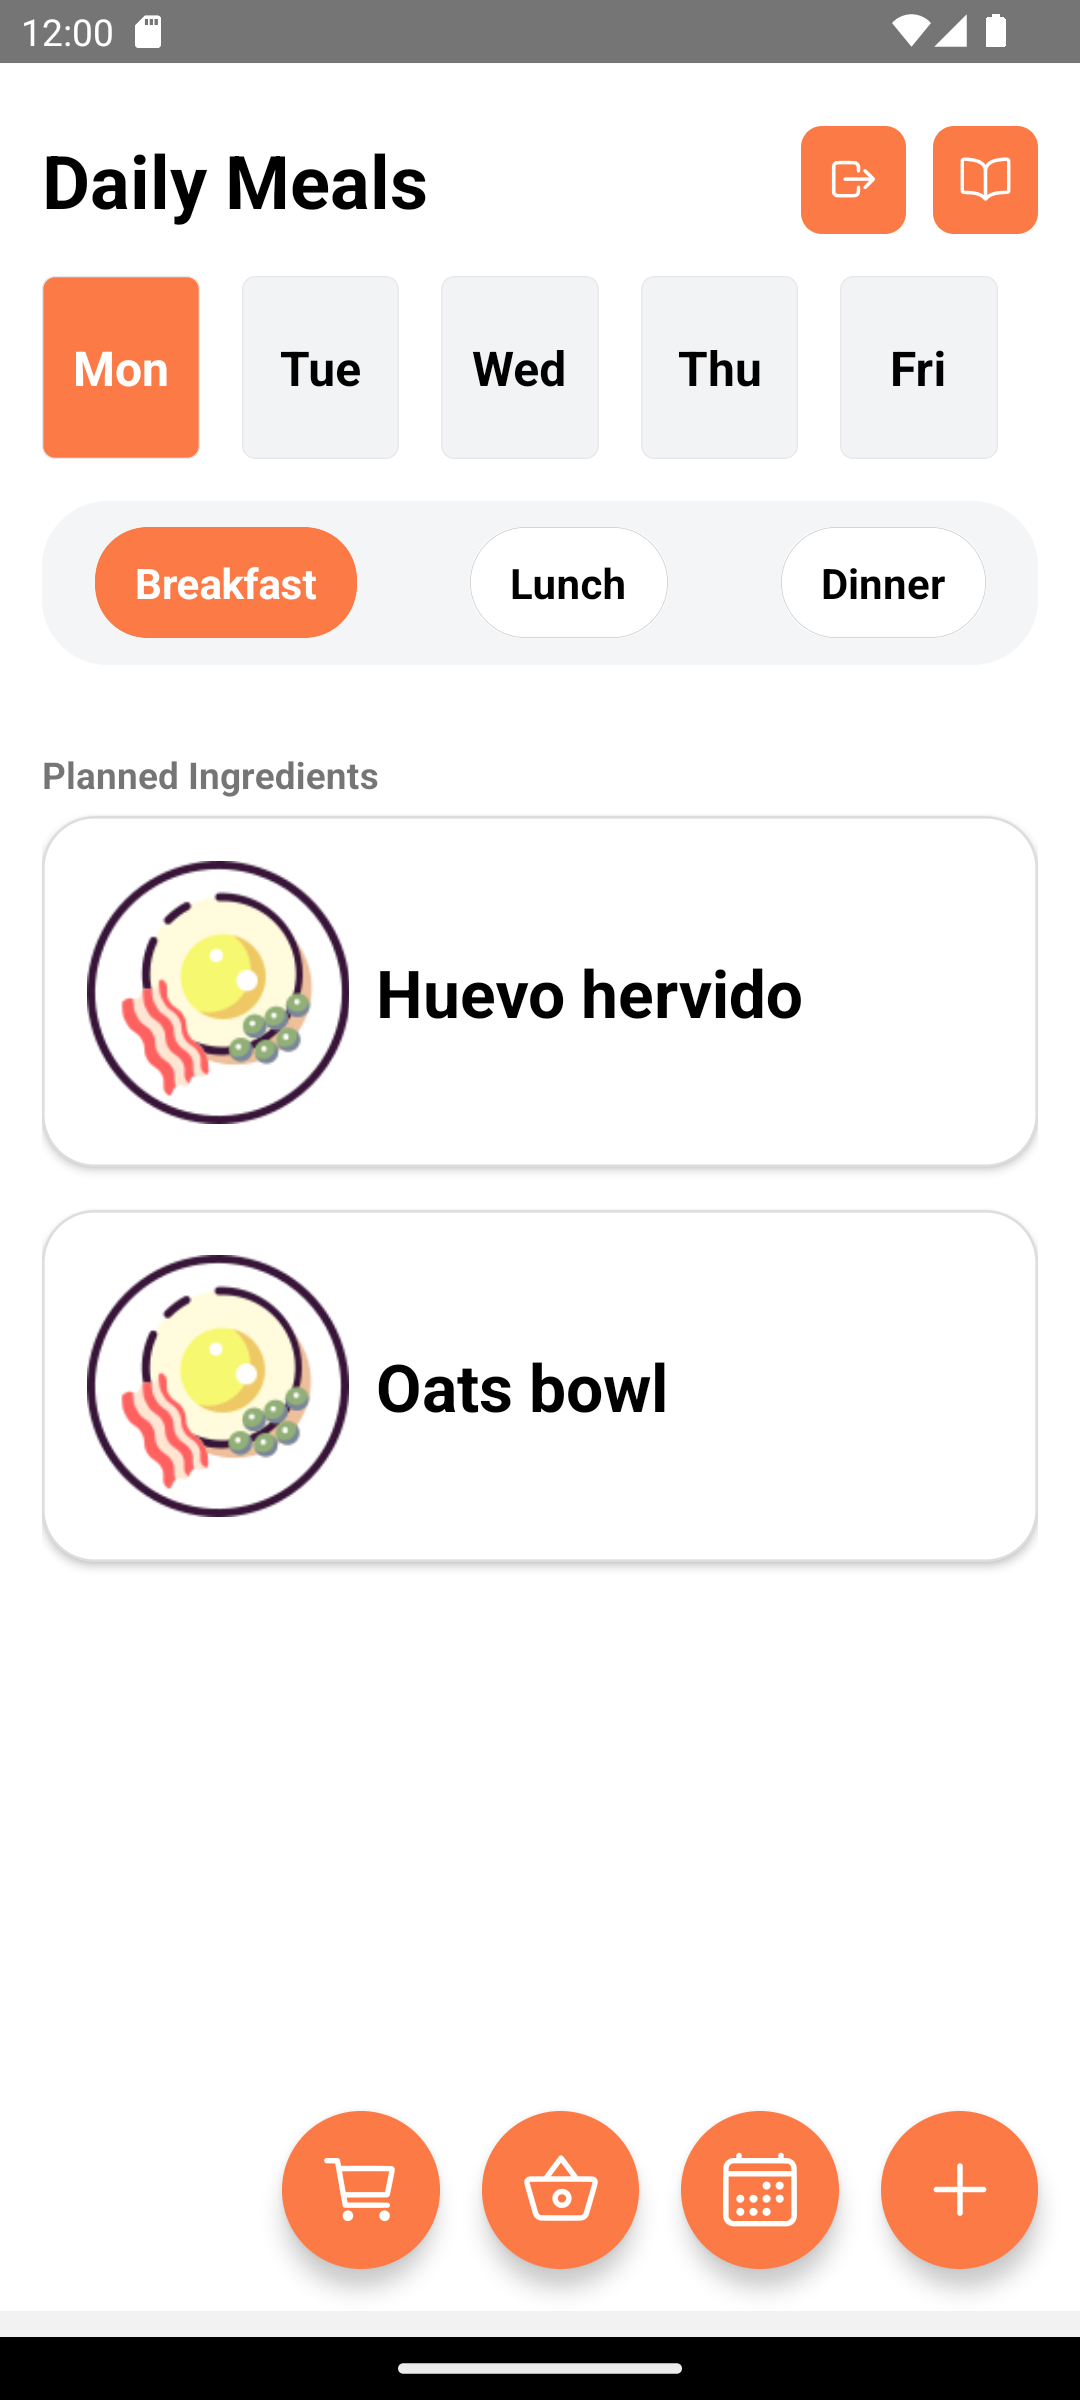
\includegraphics[scale=0.1]{imagenes/MainScreenScreenshot.png}
						\caption{\textit{Lista de \textit{PlannedIngredientCard}} modal en \hyperref[fig:MainScreen]{\textit{MainScreen} (página principal)}}
						\label{fig:PlannedIngredienCard}
					\end{figure}

				\paragraph{RecipeCardComponent}
					El \texttt{RecipeCardComponent} es la tarjeta utilizada en listados de recetas. Muestra el título, una miniatura de la imagen si existe y una breve descripción o metadato (tiempo de preparación, porciones). Las tarjetas son táctiles: un toque abre el detalle de la receta y una pulsación larga abre las opciones contextuales. La tarjeta está diseñada para priorizar la legibilidad y permitir una navegación rápida entre recetas. Es similar a PlannedIngredientCard.
						
					\begin{figure}[H]
						\centering
						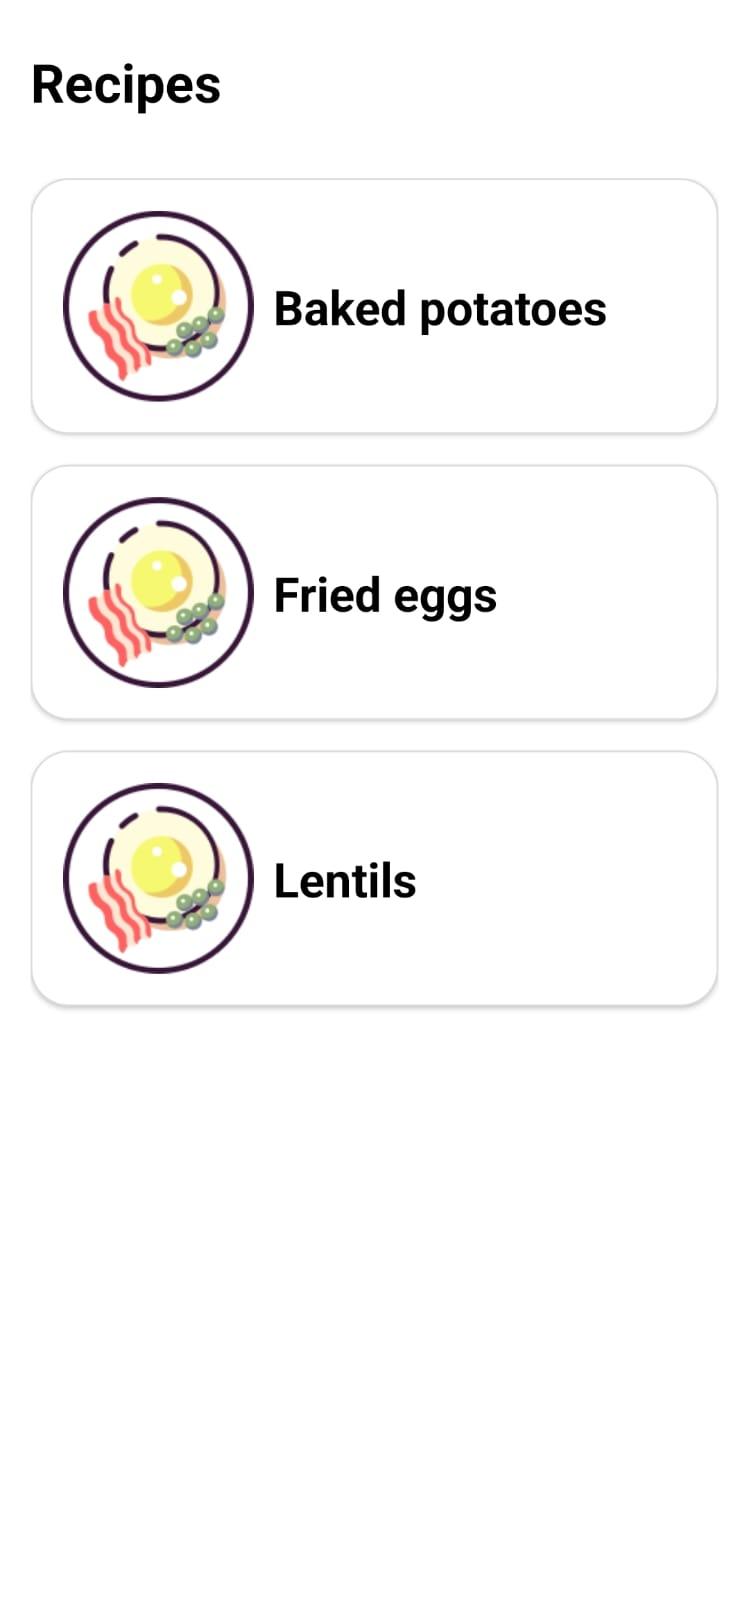
\includegraphics[scale=0.1]{imagenes/RecipesScreen.jpeg}
						\caption{\textit{Lista de \textit{RecipeCardComponent}} modal en \hyperref[fig:RecipesScreen]{\textit{RecipesScreen} (página de recetas)}}
						\label{fig:RecipeCardComponent}
					\end{figure}

				\paragraph{RecipeOptionsModal\\}
					El modal \texttt{RecipeOptionsModal} agrupa acciones contextuales sobre una receta: editar, eliminar, clonar o añadir a la planificación. Se invoca desde una pulsación larga sobre una tarjeta o desde un botón de opciones. La lógica del modal delega las operaciones al contexto o a los servicios correspondientes, mostrando confirmaciones cuando la acción es destructiva. Su objetivo es concentrar las operaciones avanzadas sin sobrecargar la vista principal.
						
					\begin{figure}[H]
						\centering
						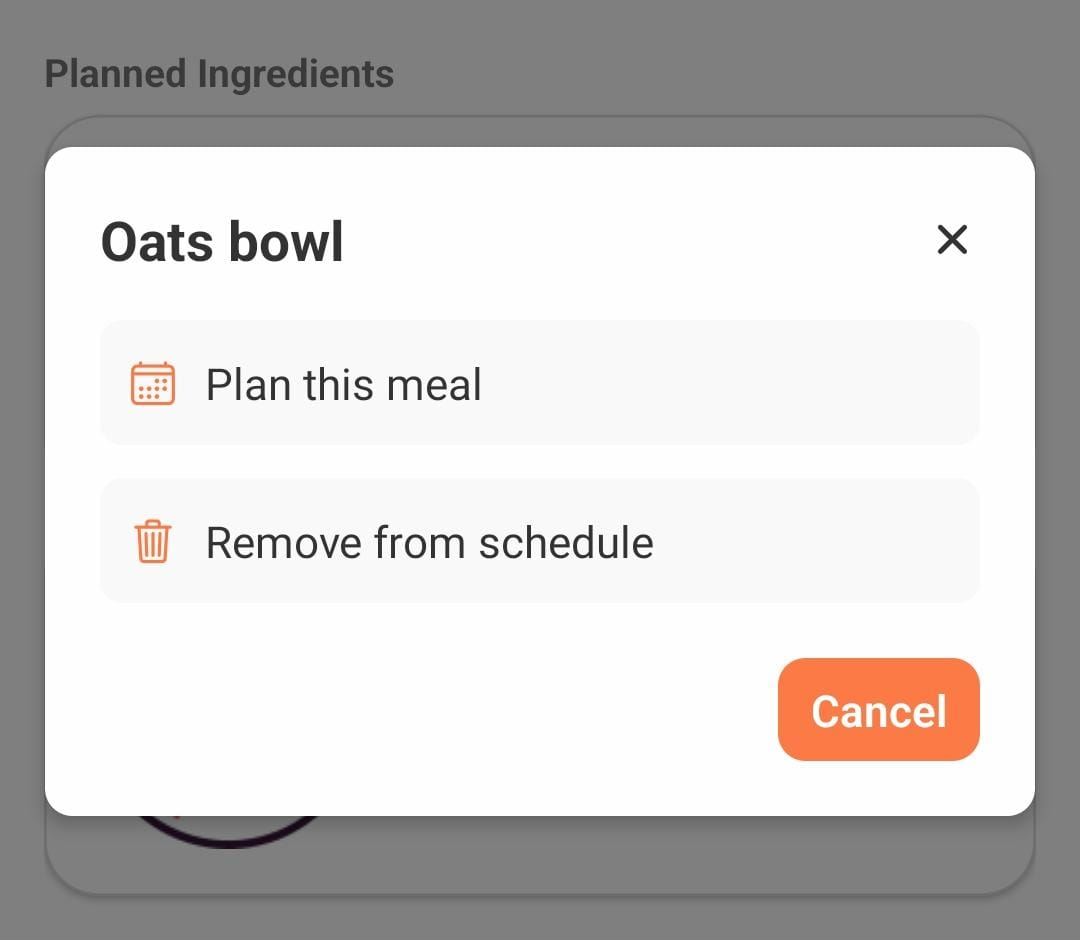
\includegraphics[scale=0.2]{imagenes/RecipeOptionsModal.jpeg}
						\caption{\textit{RecipeOptionsModal} en \hyperref[fig:MainScreen]{\textit{MainScreen}}}
						\label{fig:RecipeOptionsModal}
					\end{figure}

				\paragraph{PlanMealModal\\}
					\texttt{PlanMealModal} es el modal encargado de asignar una receta o un ingrediente a un día y tipo de comida. En su interfaz el usuario elige el día, el tipo de comida y confirma la planificación; internamente valida conflictos sencillos (por ejemplo, evitar duplicados no deseados) y delega la persistencia a los servicios de planificación. Es el punto de conexión entre la exploración de recetas y la generación del calendario semanal.
						
					\begin{figure}[H]
						\centering
						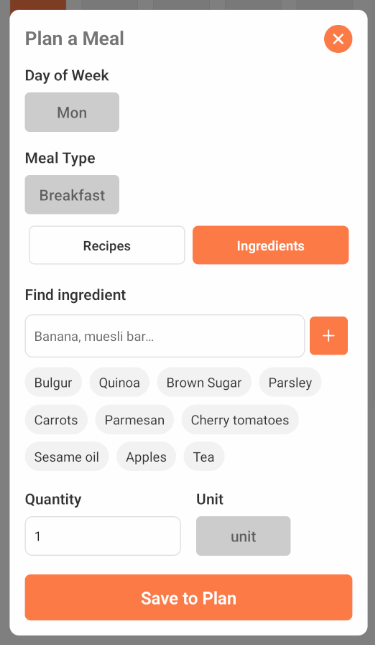
\includegraphics[scale=0.5]{imagenes/PlanMealModal.png}
						\caption{\textit{PlanMealModal} en \hyperref[fig:MainScreen]{\textit{MainScreen}}}
						\label{fig:PlanMealModal}
					\end{figure}

				\paragraph{PlannedIngredientOptionsModal}
					El modal \texttt{PlannedIngredeintOptionsModal} (nombre tal cual en el repositorio) provee opciones específicas para un ingrediente que ya forma parte de la planificación: modificar cantidad, cambiar unidad, mover a otro día o eliminar de la planificación. Centralizar estas acciones en un modal evita interfaces fragmentadas y facilita la confirmación de cambios que afectan a la lista de la compra resultante.
						
					\begin{figure}[H]
						\centering
						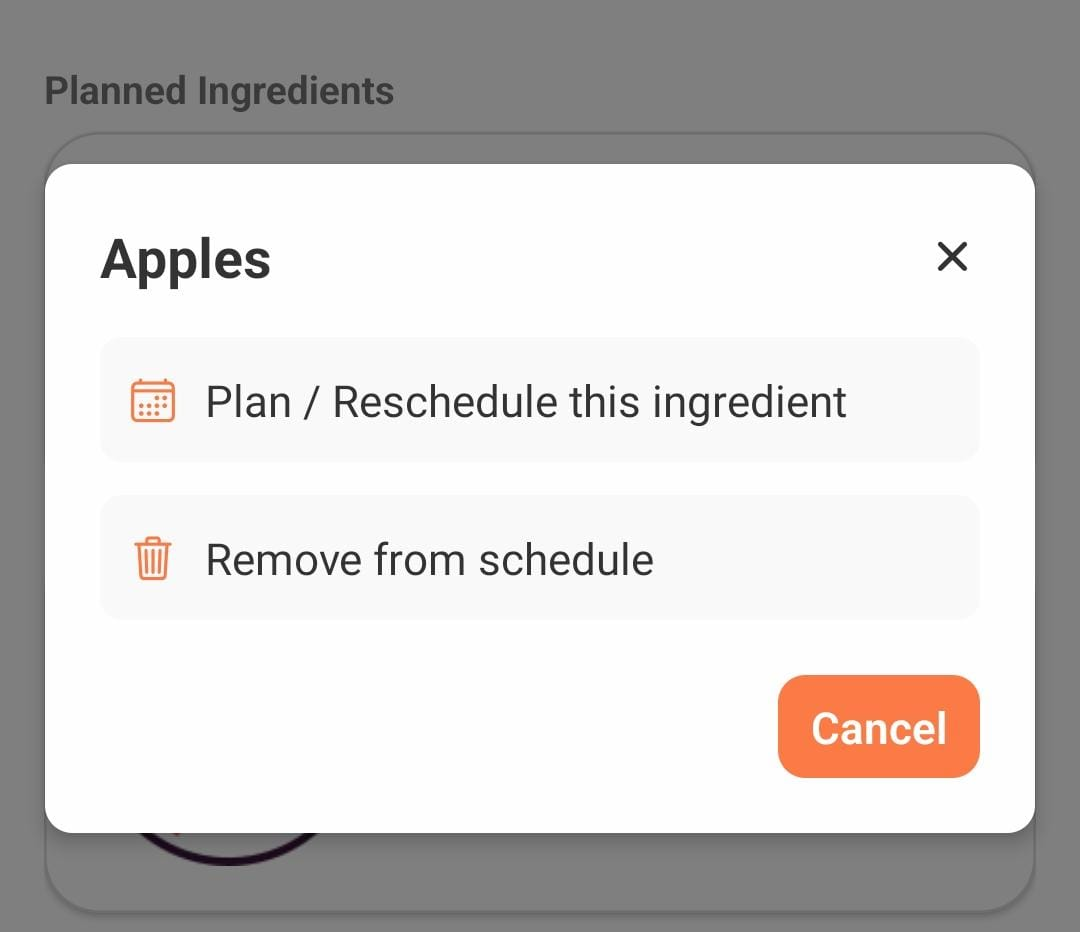
\includegraphics[scale=0.2]{imagenes/IngredientOptionsModal.jpeg}
						\caption{\textit{PlannedIngredientOptionsModal} en \hyperref[fig:MainScreen]{\textit{MainScreen}}}
						\label{fig:PlannedIngredientOptionsModal}
					\end{figure}
		\subsection{Servicios de backend (Services)}
			
				En esta sección de la aplicación se implementaron todas las funciones conectoras con la base de datos, para mejorar la legibilidad y futura mejora, se creó un archivo para cada tipo de colección creada en base de datos y cada uno de ellos tiene funciones CRUD(Create, Read, Update, Delete) de esa colección. Aparte de estos archivos, existe uno que contiene variables globales en las que se guardan los nombres de las colecciones y atributos para facilitar la programación.\\
				Las funciones CRUD son las funciones encargadas de crear, leer, actualizar y borrar una colección en Firebase. 
				
				%explicar que en Firebase no hay necesidad de crear una colección, esta se crea sola
				\subsubsection{Ingrediente (\textit{Ingredient})}
				
				En esta sección de la aplicación se implementaron todas las funciones conectoras con la base de datos; para mejorar la legibilidad y facilitar futuras mejoras, se creó un archivo por cada colección usada en la base de datos. Cada uno de estos ficheros encapsula las operaciones CRUD básicas (crear, leer, actualizar y borrar) y añade utilidades específicas necesarias por el dominio: transformación de datos entre los tipos TypeScript y la representación en Firestore, validación mínima de entradas, gestión de errores y excepciones, y logging discreto para depuración durante el desarrollo.
			
				\subsubsection{Servicio de utilidades y nombres (\texttt{db-services.tsx})}
				Este fichero centraliza los nombres de las colecciones, las constantes de campo y utilidades compartidas entre los demás servicios.  Al tener aquí las claves y nombres en un único lugar se evita la dispersión de cadenas mágicas por el código y se facilita el uso de operaciones por lotes y transacciones desde otros servicios.
				
				\subsubsection{Ingredient (\texttt{ingredient-db-services.ts})}
				Además de las CRUD habituales, el servicio de ingredientes incorpora búsquedas textuales optimizadas y lógica de deduplicación: normaliza nombres (minúsculas, eliminación de acentos) y evita inserciones redundantes. Proporciona una función que devuelve datos enriquecidos para la UI (por ejemplo, nombre, categoría y etiquetas) y un hook para reindexar el índice local de búsqueda (MiniSearch) tras modificaciones remotas, de modo que la experiencia de autocompletado sea inmediata sin depender únicamente de lecturas de la base de datos.
				
				\subsubsection{GroceryBought (\texttt{groceryBought-db-services.ts})}
				Además de almacenar y recuperar los ingredientes marcados como comprados, este servicio expone operaciones específicas para sincronizar el marcado como comprado con la despensa: al confirmar una compra puede lanzarse una operación atómica que añade o actualiza las entradas en \texttt{IngredientPantry} y registra el evento en \texttt{GroceryBought}. También incluye funciones para obtener todos los ítems comprados por periodo (por ejemplo, último mes) y para limpiar compras antiguas en bloque, operaciones pensadas para mantener coherencia entre la lista de la compra y el inventario del usuario.
				
				
				\subsubsection{IngredientPantry (\texttt{ingredientPantry-db-services.ts})}
				Este servicio realiza operaciones sobre el inventario del usuario que van más allá del simple get/set: suma y resta de cantidades con verificación de unidades, consolidación de filas duplicadas y transferencias entre entradas (p. ej. al marcar comprado). Implementa actualizaciones idempotentes y operaciones en lote para asegurar que varias modificaciones relacionadas (restar de una fila, añadir en otra) se apliquen de forma consistente; cuando procede usa transacciones para evitar condiciones de carrera en escenarios concurrentes.
				
				\subsubsection{Recipe (\texttt{recipe-db-services.ts})}
				Las funciones especiales de este servicio incluyen la recuperación de recetas filtradas por \texttt{userId} (garantizando multiusuario), la subida y asociación de imágenes (gestión de rutas/URL) y la clonación de recetas para facilitar plantillas o importaciones. También expone una operación compuesta que crea la receta y sus \texttt{RecipeIngredient} asociados en una sola secuencia controlada, devolviendo la entidad completa ya lista para mostrarse en la UI.
				
				\subsubsection{RecipeIngredients (\texttt{recipeIngredients-db-services.ts})}
				Aquí se implementan utilidades para obtener todos los ingredientes de una receta con sus nombres resueltos, para agregar o eliminar listas completas de ingredientes cuando se edita una receta y para agrupar cantidades por unidad cuando se generan cálculos (por ejemplo, sumar gramos de un mismo ingrediente). Dispone de funciones de batch para crear o borrar múltiples \texttt{RecipeIngredient} manteniendo la integridad referencial con la receta padre.
				
				\subsubsection{WeeklyMeals (\texttt{weeklyMeals-db-services.ts})}
				Más allá de las operaciones CRUD puntuales, este servicio contiene las rutinas que permiten extraer todos los ingredientes necesarios para la planificación semanal: convierte entradas tipo receta en sus ingredientes desglosados, agrega cantidades iguales por unidad y proporciona una API para obtener los datos ya agrupados por día y tipo de comida. También soporta consultas por \texttt{userId} y por rango de fechas, y ofrece una función que valida que no existan solapamientos o duplicados en un mismo día/comida antes de escribir nuevos \texttt{WeeklyMeal}.
				

				
		\subsection{Contexto (Context)}
				En NutriPlan, el contexto (\texttt{Context.tsx}) actúa como una capa intermedia entre los servicios de Firebase y la interfaz de usuario, centralizando el estado global de la aplicación y proporcionando métodos para su manipulación.\\
				\textbf{\\Diseño del contexto}\\
				El contexto se implementó siguiendo un patrón de diseño que separa la definición de tipos, el estado inicial y los métodos de manipulación. Esta separación facilita el mantenimiento y la escalabilidad del código. El contexto mantiene en memoria:
				
				\begin{itemize}
					\item Lista completa de ingredientes para búsquedas rápidas
					\item Recetas del usuario actual
					\item Estado de la despensa
					\item Planificación semanal activa
					\item Elementos marcados como comprados
				\end{itemize}
				
				\textbf{\\Integración con Firebase}\\
				El contexto abstrae la complejidad de las operaciones con Firebase mediante métodos que encapsulan las llamadas a los servicios. Por ejemplo, cuando un componente necesita añadir una receta, invoca \texttt{addRecipe} del contexto en lugar de interactuar directamente con \texttt{recipe-db-services}. Este enfoque tiene varias ventajas:
				
				\begin{itemize}
					\item Centraliza la lógica de actualización de estado
					\item Reduce la duplicación de código en componentes
					\item Facilita la implementación de caché y optimizaciones
					\item Simplifica el testing al poder mockear el contexto
				\end{itemize}
				
				\textbf{\\Gestión de estado global}\\
				El contexto implementa un sistema de suscripción que notifica a los componentes cuando los datos relevantes cambian. Por ejemplo, cuando se marca un ingrediente como comprado en \texttt{GroceryListScreen}, el contexto:
				
				\begin{enumerate}
					\item Actualiza el estado en Firebase mediante \texttt{groceryBought-db-services}
					\item Modifica el estado local para reflejar el cambio
					\item Notifica a los componentes suscritos (como la lista de la compra y la despensa)
				\end{enumerate}
				
				\textbf{\\Inicialización y ciclo de vida}\\
				Como se observa en \texttt{App.tsx}, el contexto se inicializa al arrancar la aplicación mediante \texttt{AppProvider}, que envuelve toda la navegación. Esta disposición garantiza que el estado global está disponible en cualquier pantalla y que la autenticación del usuario (\texttt{FirebaseAuth}) está correctamente integrada con el resto de la aplicación.
				\\\\
				El diseño del contexto prioriza la eficiencia y la simplicidad, siguiendo los mismos principios minimalistas que guían el resto de la aplicación. La decisión de usar Context API de React en lugar de soluciones más complejas como Redux se alinea con el objetivo de mantener la base de código simple y mantenible, mientras se satisfacen las necesidades de estado global de la aplicación.
	
	
	\section{Mockups}
	%Explicar el diseño de la interfaz gráfica
	\section{Conclusiones}

\chapter{Prototipos y desarrollo}\label{cap.prototipos y desarrollo}
%Poner tantos prototipos como estimes necesario. En cada prototipo, meter alguna funcionalidad o completar alguna parte de la aplicación. Si mejoramos mucho algo, crear un prototipo nuevo.
  \section{Prototipo 1}
  \section{Prototipo 2}
  \section{Prototipo 3}
  \section{Conclusiones}

\chapter{Conclusiones y mejoras futuras}\label{cap.conclusiones y mejoras futuras}
  \section{Conclusiones técnicas}
  %Hablar desde el punto de vista del software de aspectos como el hecho de lo que nos ayuda React-Native
  \section{Conclusiones personales}
  %Valoración personal sobre cada una de las cosas vistas durante el proyecto
  \section{Futuras mejoras}
  %Trabajos futuros que se puedan relacionar con este

\chapter{Conclusions and future works}\label{cap.conclusions and future works}
  \section{Technical conclusions}
  \section{Personal conclusions}
  \section{Future works}

\cleardoublepage
\addcontentsline{toc}{chapter}{Bibliografía}
\bibliographystyle{acm} % estilo de la bibliografía.
\bibliography{citas} % citas.bib es el fichero donde está salvada la bibliografía.



\end{document}
